%\documentclass[9pt,twocolumn,twoside]{IEEEtran} 
%\documentclass[9pt]{article}
\documentclass[landscape,letterpaper,9pt]{article}
%unix>  latex landscapedoc.tex                   (creates land.dvi)
%unix>  xdvi  -paper usr  landscapedoc.dvi       (preview DVI file)
%unix>  dvips -Ppdf  -t landscape  landscapedoc.dvi    (creates land.ps)
%unix>  ghostview  -landscape  landscapedoc.ps   (preview PostScript file)
%unix>  ps2pdf  landscapedoc.ps                  (creates land.pdf)
%
%
%%\documentstyle[twocolumn,twoside]{IEEEtran}
\usepackage{graphicx,multirow}%hbaw,pstricks}
\usepackage{color,pstcol}
\usepackage{srcltx,xr}
%\usepackage[baw,pstricks]{fvrb-ex}
%\documentclass[a4paper,12pt]{slides}
%\usepackage[html,4]{tex4ht}
%\usepackage{latexcad}
\usepackage{amsmath,fvrb-ex,bm,ee}
%\usepackage{srcltx}
\usepackage{amsfonts}
\usepackage{amssymb}
\usepackage{amsthm}
\usepackage{newlfont}
%\usepackage{pst-all}      % From PSTricks
%\usepackage{pst-poly}     % From pstricks/contrib/pst-poly
%\usepackage{multido}      % From PSTricks
%\usepackage{pstcol}      % From PSTricks
%\title{\color{blue}Latex Support Test File}
%\author{\color{green}Mark A. Wicks}
\def\stackunder{\stackrel}
\setlength{\footnotesep}{15pt} \setlength{\topmargin}{0in}
\setlength{\textwidth}{6.25in} \setlength{\oddsidemargin}{0in}
\setlength{\evensidemargin}{0in} \setlength{\textheight}{8in}
\fvset{gobble=0,numbersep=3pt}
\fvset{numbers=left,frame=single}
\RecustomVerbatimEnvironment{Verbatim}{Verbatim}{commandchars=???}
\DefineVerbatimEnvironment%
{CVerbatim}{Verbatim}
  {fontfamily=tt,fontsize=\small,commandchars=\\\{\},commentchar=\?,frame=single,formatcom=\color{midnightblue},label=\emph{Interactive R example}}
\DefineVerbatimEnvironment{Sinput}{Verbatim}{fontshape=sl,formatcom=\color{midnightblue}}


\makeatother

\setlength{\oddsidemargin}{0in}     % default=0in 
\setlength{\textwidth}{9.5in}     % default=9in

\setlength{\columnsep}{0.5in}       % default=10pt
\setlength{\columnseprule}{1pt}     % default=0pt (no line)

\setlength{\textheight}{5.85in}     % default=5.15in
\setlength{\topmargin}{-0.35in}     % default=0.20in
\setlength{\headsep}{0.25in}        % default=0.35in

\setlength{\parskip}{1.2ex} \setlength{\parindent}{0mm}
% This for broken installs that flip page wrong way
\special{! TeXDict begin /landplus90{true}store end }

\definecolor{midnightblue}{rgb}{0.098,0.098,0.439}
\definecolor{darkyellow}{rgb}{1, 0.9, 0}
\newcommand\cbox[1]{\colorbox{darkyellow}{#1}}

\begin{document}
%\maketitle
\let\Footnotesize=\large
\let\Tiny=\large
\let\small=\Large
\let\normalsize=\LARGE
\let\large=\Large
\let\Large=\Large

\sffamily
\large
\newcommand{\us}[2]{\ensuremath{\underset{\left(#2\right)}{#1}}}



\input eda_2010
\begin{center}
\textbf{Notes on  Panel Data Analysis}
\end{center}

\vspace{0.2in}
%``\emph{For d'ye see, rainbows do not visit the clear
%air; they only irradiate vapor}"
%(Melville, Moby Dick).

"\textit{I see that you are an enthusiast of this new science. Would you care to try another word? Trash.}"

"\textit{Why not? It doesn't matter that you're a skeptic. Not in the least. What was it again, trash? Very well ... trash,
trashcan, ashcan, trashman. Trashmass, trashmic, catatrashmic. Trashmass, trashmosh.
In a large enough scale, trashmos. And-of course - macrotrashm! Tichy, you come up with the best words!
Really, just think of it, macrotrashm!}"

"\textit{I'm afraid I don't follow. It's nonsense to me.}" ...

``\textit{Secondly, macrotrashm is nonsense so far, yet we can already guess its sense-to-be,
its future significance.
The word observe, implies nothing less than a new psychozoic theory!
Implies that the stars are of artificial origin!}"

"\textit{Now where do you get that?}"

"\textit{From the word itself. Macrotrasm indicates, or rather suggests, this image:
in the course of many eons the Universe filled up with trash, the wastes of various
civilizaitons. The wastes got in the way, of course, hampering astronomers and cosmonauts,
and so enormous incinerators were built, all at extremely high temperatures, observe, to
burn the trash, and with sufficient mass to pull it in from space themselves.
Gradually space clears up and behold, there are your stars, those selfsame furnaces,
and the dark nebulae-this is the trash that remains to be removed.}"

"\textit{You can't be serious! The Universe nothing but one big trash disposal?
You don't really think that's possible? Professor!}"
(The Futurological Congress, Lem, 1974)

%\begin{itemize}
%\item Aims
%\begin{itemize}
%\item The aim of these lectures to enable students to explore the
%relationship between steadily increasing incomes and environmental quality.
%\end{itemize}
%
%\item Learning Outcomes
%\begin{itemize}
%\item Understand relationship between steadily increasing incomes and environmental quality.
%\item Use panel data regression techniques.
%\item Understand assumptions, strengths and weaknesses, and appropriate uses of panel methods.
%\item Know how quantities needed for policy analysis are computed from regression results.
%\end{itemize}
%\end{itemize}
\newpage
%\large \sffamily
\vspace{0.2in}
\tableofcontents
\vspace{0.2in}
\newpage
\section{Independently Pooled Cross Sections}
\begin{itemize}
    \item If a random sample from a population is obtained at different points in
    time we obtain an \emph{independently pooled cross section}.
    \item To account for the possibility of differently distributed populations in different years,
    time dummies are usually included.
\end{itemize}
\subsection{Policy Analysis with Pooled Cross Sections}
Independently pooled cross sections can  be used to analyze so-called \emph{natural experiments}.
A natural experiment occurs when there is an exogenous source of variation in the explanatory
variables, i.e., when, say because of a policy change, the environment in which individuals,
households, firms, countries,  etc., operate,  is changed.
A natural experiment will always determine a
\emph{control group}, not affected by the policy change,
and a \emph{treatment group}, which is considered affected by the change.
This occurrence is particularly useful wherever estimates seem particularly susceptible to
omitted variable bias. For instance, consider the impact on house prices of the
construction of a new incinerator.
It is very likely that the incinerator will be build in areas where the house prices are
already low, and are likely to remain low after the construction of the incinerator.
A standard OLS regression would incorrectly attribute this difference in prices to the effect of
the incinerator, and hence bias the estimated coefficient.

\newpage
\subsection{Difference--in--Difference (DD) Estimator}
DD estimation consists of identifying a policy intervention (treatment) and then compare the difference
in outcomes after and before the intervention for the groups affected by it to this difference for
unaffected groups. In order to control for preexisting heterogeneity between control and treatment groups,
at least two years of data are required, one before the policy intervention ad one after.

\newpage
\subsection{The Case of an Incinerator}

%
%\setlength{\unitlength}{1mm}
% \input{incin.lp}

\subsubsection{Data}
%\renewcommand{\FancyVerbFormatLine}[1]{%
%  \ifnum\value{FancyVerbLine}<5\color{red}#1%
%  \else\color{blue}#1\fi}
\begin{CVerbatim}
\fbox{line} 1
line 2
line 3
line 4
line 5
line 6
line 7
\end{CVerbatim}

\begin{itemize}
\item
Kiel and McClain (1995): ``House Prices  During  Siting  Decisions Stages: The Case of an Incinerator
from Rumor Through Operation," \emph{Journal of Environmental Economics and Management}, 28, 241--255.
\end{itemize}
\begin{Verbatim}
year      age       agesq     nbh       cbd       intst     lintst    price
rooms     area      land      baths     dist      ldist     wind      lprice
y81       larea     lland     y81ldist  lintstsq  nearinc   y81nrinc  rprice
lrprice

  Obs:   321

  1. year                     1978 or 1981
  2. age                      age of house
  3. agesq                    age^2
  4. nbh                      neighborhood #, 1 to 6
  5. cbd                      dist. to central bus. dstrct, feet
  6. intst                    dist. to interstate, feet
  7. lintst                   log(intst)
  8. price                    selling price
  9. rooms                    # rooms in house
 10. area                     square footage of house
 11. land                     square footage lot
 12. baths                    # bathrooms
 13. dist                     dist. from house to incinerator, feet
 14. ldist                    log(dist)
 15. wind                     perc. time wind incin. to house
 16. lprice                   log(price)
 17. y81                      =1 if year == 1981
 18. larea                    log(area)
 19. lland                    log(land)
 20. y81ldist                 y81*ldist
 21. lintstsq                 lintst^2
 22. nearinc                  =1 if dist <= 15840
 23. y81nrinc                 y81*nearinc
 24. rprice                   price, 1978 dollars
 25. lrprice                  log(rprice)
\end{Verbatim}
\newpage
\subsubsection{Estimations}
\begin{itemize}
    \item Consider the model for 1981
\[ rprice_{i,1981} = \alpha_1 + \alpha_2 \;  nearinc_{i,1981} + \epsilon_{i,1981} \]
where \(nearinc\) is a dummy defined as

\[
nearinc =
\begin{cases}
    1, &\text{if $distance \leq 15840$ feet}; \\
    0, &\text{otherwise}.
\end{cases}
\]

\item What is the interpretation of the OLS estimators \(\widehat{\alpha}_1\) and \(\widehat{\alpha}_2\)?
\item
%The equation basically states that the a house price in 1981 is given by t
\(\widehat{\alpha}_1\) estimates the 1981 average price of all houses distant from the incinerator,
\(\widehat{\alpha}_1 + \widehat{\alpha}_2\) estimates the 1981 average price of all houses near to the incinerator,

\[\widehat{\alpha}_1 = \overline{rprice}_{1981,nearinc=0},\]
\[\widehat{\alpha}_1 + \widehat{\alpha}_2 = \overline{rprice}_{1981,nearinc=1},\]
and hence \(\alpha_2\) estimates the 1981 difference in average price between  houses that
are distant and those that are close to the incinerator,\footnote{When regressing rprice on a constant,
OLS yields the sample average of \textit{rprice} as the fitted coefficient. OLS will
return the value of \(\alpha_1\) that
\[
\min_{\alpha_1} S( \alpha_1) = \sum_{i=1}^n (rprice_i - \alpha_1)^2,
\]
i.e, the solution to
\[
\frac{\partial S(\alpha_1) }{\partial \alpha_1} = \sum_{i=1}^n  - 2 (rprice_i - \alpha_1)=0,
\]
\[
 \sum_{i=1}^n  rprice_i  =  \sum_{i=1}^n  \alpha_1,
\]

\[
\sum_{i=1}^n  rprice_i  =  n  \alpha_1,
\]
\[
\alpha_1 = \frac{1}{n} \sum_{i=1}^n  rprice_i = \overline{rprice}.
\]
If we add the incinerator indicator, \textit{nearinc},  the minimization becomes
\[
\min_{\alpha_1, \alpha_2} S( \alpha_1,\alpha_2) = \left\{ \sum_{i=1}^n (rprice_i - \alpha_1 - \alpha_2 nearinc)^2 \right\},
\]
which can be rewritten as
\[
\min_{\{\alpha_1, \alpha_2\}} S( \alpha_1,\alpha_2) = \left\{ \sum_{\{i| nearinc=0\}} (rprice_i - \alpha_1)^2 +
 \sum_{\{i| nearinc=1\}} (rprice_i - \alpha_1 - \alpha_2 nearinc)^2 \right\}=
\]
\[
=\left\{ \min_{\{\alpha_1, \alpha_2\}}  \sum_{\{i| nearinc=0\}} (rprice_i - \alpha_1)^2\right\} +
\left\{  \min_{\{\alpha_1, \alpha_2\}}   \sum_{\{i| nearinc=1\}} (rprice_i - \alpha_1 - \alpha_2)^2 \right\}=
\]
\[
=\left\{ \min_{\{\alpha_1, \alpha_2\}}  \sum_{\{i| nearinc=0\}} (rprice_i - \alpha_1)^2\right\} +
\left\{  \min_{\{\alpha_1, \alpha_2\}}   \sum_{\{i| nearinc=1\}} (rprice_i  - \gamma)^2 \right\}
\]
so that the fitted value of \(\alpha_1\) is the average of prices for homes close to the incinerator only, the fitted value
of \(\alpha_1+\alpha_2 = \gamma\) is the average of home prices far from the incinerator, and, therefore
the fitted value for \(\alpha_2\) is the difference in home's average prices for distant and the average for close
to the incinerator.
}
\[\widehat{\alpha}_2 = \overline{rprice}_{1981,nearinc=1} - \overline{rprice}_{1981,nearinc=0}.\]

\end{itemize}

\begin{CVerbatim}
dd <- read.table("e:/statmeth/KIELMC.dat", header=T)
> names(dd)
 [1] "year"     "age"      "agesq"    "nbh"      "cbd"      "intst"    "lintst"   "price"
 [9] "rooms"    "area"     "land"     "baths"    "dist"     "ldist"    "wind"     "lprice"
[17] "y81"      "larea"    "lland"    "y81ldist" "lintstsq" "nearinc"  "y81nrinc" "rprice"
[25] "lrprice"
> attach(dd)

> lm( rprice ~ nearinc, data = subset(dd, year==1981) )

Call:
lm(formula = rprice ~ nearinc, data = subset(dd, year == 1981))

Coefficients:
(Intercept)      nearinc
     101308       -30688
\end{CVerbatim}

\newpage
Estimation Results
\begin{enumerate}
\item[(i)] The fitted regression line is
\[\widehat{rprice} = \us{101307.5145}{32.754} - \us{30688.27376}{-5.266}\; nearinc \]
\item[(ii)] The negative coefficient for \emph{nearinc} suggests, as
expected from  ``theory,'' that being close to the incinerator lowers house values.
\item[(iii)] We estimate that being close to the incinerator  determines a fall of
\$30688.27376 in the average selling price of homes. Figure~\ref{fig:hou1} illustrates the regression results.

%
%\begin{center}
%\begin{figure}[h!]
%\caption{Regression for 1981\label{fig:hou1}}
%%   \vspace{.1in}
%  \centering \leavevmode 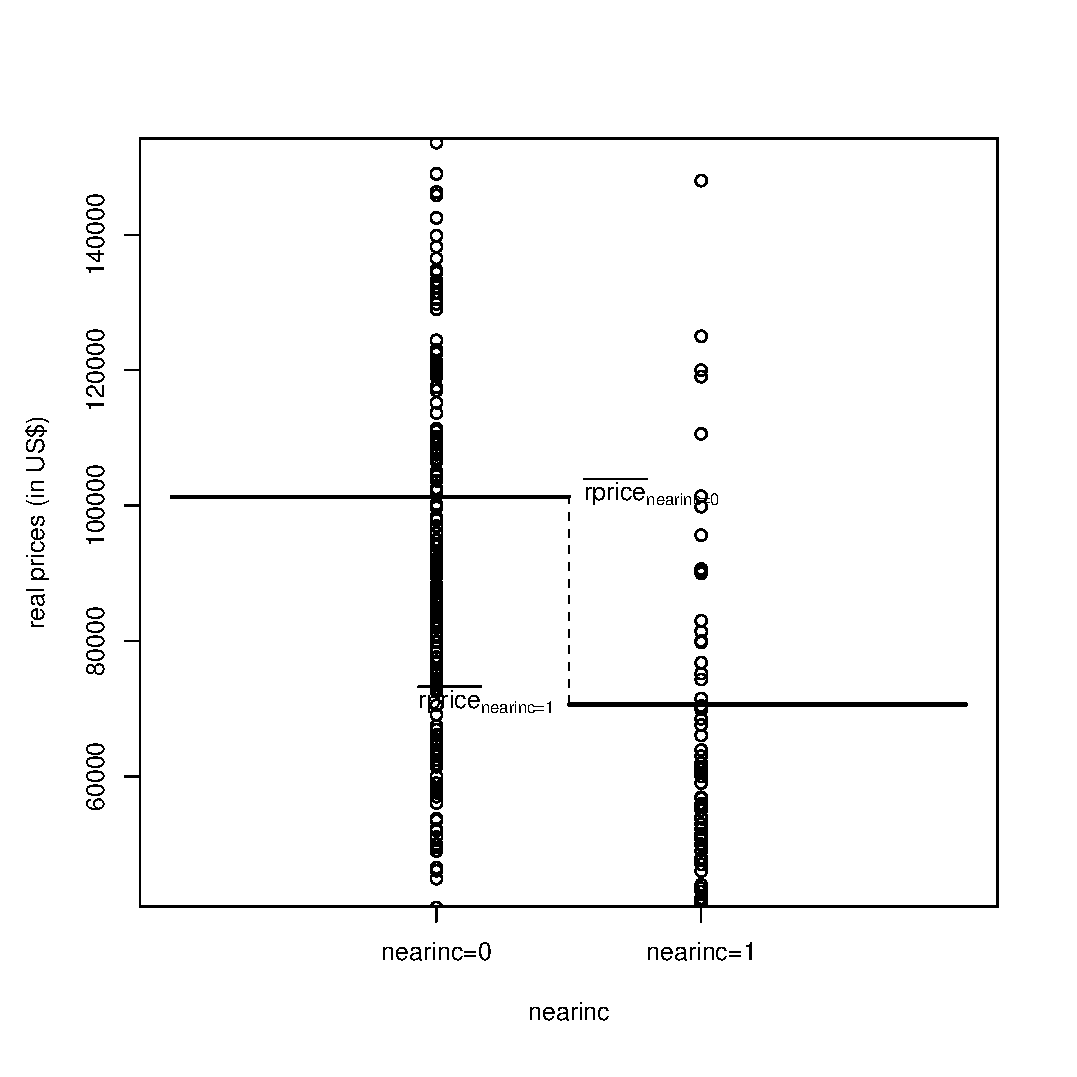
\includegraphics[angle=0,width=3.5in]{aee_hou1.ps}
%\end{figure}
%\end{center}

\end{enumerate}

\newpage
Model for 1978
\[ rprice_{i,1978} = \beta_1 + \beta_2 \;  nearinc_{i,1978} + \epsilon_{i,1978} \]

\begin{itemize}
\item What is the interpretation of the OLS estimators \(\widehat{\beta}_1\) and \(\widehat{\beta}_2\)?
\item Analogously to the 1981 case,
\[\widehat{\beta}_1 = \overline{rprice}_{1978,nearinc=0},\]
\[\widehat{\beta}_1 + \widehat{\beta}_2 = \overline{rprice}_{1978,nearinc=1},\]
and hence
\[\widehat{\beta}_2 = \overline{rprice}_{1978,nearinc=1} - \overline{rprice}_{1978,nearinc=0}.\]
\end{itemize}

\begin{CVerbatim}
> lm( rprice ~ nearinc, data = subset(dd, year==1978) )

Call:
lm(formula = rprice ~ nearinc, data = subset(dd, year == 1978))

Coefficients:
(Intercept)      nearinc
      82517       -18824
\end{CVerbatim}

\newpage
Estimation Results
\begin{enumerate}
\item[(i)] The fitted regression line is
\[\widehat{rprice} = \us{82517.22764}{31.094} - \us{18824.37050}{-3.968 }\; nearinc \]
\item[(ii)] The negative coefficient for \emph{nearinc} suggests that being close to the
``to be build" incinerator has a negative impact
on home values. How can we interpret this findings?
\item[(iii)] We estimate that being close to the ``to be constructed" incinerator  determines a fall of
\$18824.37050 in the average selling price of homes.


\end{enumerate}
\newpage
\subsubsection{Economic Significance}
The impact of the construction of the incinerator on values of homes is given by
\[\widehat{ \delta} = \widehat{\alpha}_2-\widehat{\beta}_2 = -30688.27376  - (-18824.37050 ) = -11863.90 dollars\]
which is also known as the \emph{difference-in-differences estimator} as it can be expressed as
a difference of differences
\[
\widehat{\delta} =
\left( \overline{rprice}_{1981,nearinc=1} - \overline{rprice}_{1981,nearinc=0} \right) -
\left( \overline{rprice}_{1978,nearinc=1} - \overline{rprice}_{1978,nearinc=0} \right)
\]

\newpage
\subsubsection{Statistical Significance}
To test whether the impact is significantly different from zero, \(\rH_0\!\!: \delta =0\),  we need the standard
error (square root of the variance)
 of \(\widehat{\delta}\).
%
%The variance of a difference between, \(\widehat{\alpha}_2\) and \(\widehat{\beta}_2\),  is given by
%\[\var(\widehat{\delta}) = \var(\widehat{\alpha}_2-\widehat{\beta}_2) =
%\var(\widehat{\alpha}_2) + \var(\widehat{\beta}_2) - 2 \cov(\widehat{\alpha}_2,\widehat{\beta}_2).\]
%Once we estimated two separate models, we do not have the covariance.
%We need another approach.
%
We can estimate the following pooled model

\[ rprice = \gamma_1 + \gamma_2 \; y81 + \gamma_3 \; nearinc  + \delta  \; (y81 \cdot nearinc) + \nu \]

\[\frac{\partial rprice}{\partial  nearinc} =
\begin{cases}
    \gamma_3 + \delta , &\text{if $year=81$}; \\
     \gamma_3 , &\text{if $year=78$}.
\end{cases}
\]

\[intercept =
\begin{cases}
    \gamma_1 + \delta , &\text{if $year=81$}; \\
     \gamma_3 , &\text{if $year=78$}.
\end{cases}
\]



\begin{table}[h!]\caption{Summary of impacts}\label{tab:imp}
     \begin{center}
        \begin{tabular}{|c|c|c|c}\hline
             & $nearinc=1$           & $nearinc=0$ \\ \hline
     year=78 & $\gamma_1+\gamma_3$ & $\gamma_1$ \\ \hline
     year=81 & $\gamma_1+\gamma_2 +\gamma_3 + \delta$ & $\gamma_1 + \gamma_2$ \\
    \hline
\end{tabular} \vspace{-.2in}
\end{center}
\end{table}
%\clearpage
\newpage
\[ rprice = \gamma_1 + \gamma_2 \; y81 + \gamma_3 \; nearinc  + \delta  \; (y81 \cdot nearinc) + \nu \]

\[\frac{\partial rprice}{\partial  nearinc} =
\begin{cases}
    \gamma_3 + \delta \;y81, &\text{if $nearinc=1$}; \\
     \gamma_1 + \gamma_2 y81  , &\text{if $nearinc=0$}.
\end{cases}
\]

\begin{table}[h!]\caption{Summary of impacts}\label{tab:imp}
     \begin{center}
        \begin{tabular}{|c|c|c|c}\hline
             & $nearinc=1$           & $nearinc=0$ \\ \hline
     year=78 & $\gamma_1+\gamma_3$ & $\gamma_1$ \\ \hline
     year=81 & $\gamma_1+\gamma_2 +\gamma_3 + \delta$ & $\gamma_1 + \gamma_2$ \\
    \hline
\end{tabular} \vspace{-.2in}
\end{center}
\end{table}
Note that (from Table~\ref{tab:imp}):
\begin{itemize}
\item \(\gamma_1\) captures the house prices for  houses far from  the incinerator in  1978.
\item \(\gamma_2\) captures the change in house prices for all houses from 1978 to 1981.
\item \(\gamma_3\) captures the effect of the location of the house not due to the presence of
 the incinerator.
\end{itemize}
Omitting any of the two dummies can bias \(\delta\).
\newpage
\begin{CVerbatim}
> lm( rprice ~ y81 + nearinc + y81nrinc, data = dd )

Call:
lm(formula = rprice ~ y81 + nearinc + y81nrinc, data = dd)

Coefficients:
(Intercept)          y81      nearinc     y81nrinc
      82517        18790       -18824       -11864

\end{CVerbatim}
%
%Note how the estimate in the interaction term \(y81nrinc\) changes  when either
%\(y81\) or \(nearinc\).
%%
%\begin{Verbatim}
%> lm( rprice ~ y81 + y81nrinc, data = dd )
%
%Call:
%lm(formula = rprice ~ y81 + y81nrinc, data = dd)
%
%Coefficients:
%(Intercept)          y81     y81nrinc
%      76628        24679       -30688
%\end{Verbatim}
%
%
%\begin{CVerbatim}
%> lm( rprice ~  nearinc +  y81nrinc, data = dd )
%
%Call:
%lm(formula = rprice ~ nearinc + y81nrinc, data = dd)
%
%Coefficients:
%(Intercept)      nearinc     y81nrinc
%      91035       -27343         6926
%\end{CVerbatim}
%\clearpage
%\newpage
%\subsection{Chow Test}
%The Chow test is used to test whether a regression  function differs across two groups or time periods.
%It is an \emph{F} test, and as such, requires residual sums of squares from an unrestricted and a restricted regression.
%Suppose, the regressions for the two periods are
%\begin{equation}\label{eq:rss1a}
%\text{period 1:} \qquad y_i = \alpha_1 +  \alpha_2 x_{i1} + \ldots +  \alpha_k x_{ik} +  \epsilon_{i1} \qquad \text{\textbf{UR}}
%\end{equation}
%\begin{equation}\label{eq:rss2a}
%\text{period 2:} \qquad  y_i = \beta_1 +  \beta_2 x_{i1} + \ldots +  \beta_k x_{ik} +  \epsilon_{i2}\qquad \text{\textbf{UR}}
%\end{equation}
%and \(n_1\) and \(n_2\) are the number of observations in the two periods.
%\begin{itemize}
%    \item To obtain the unrestricted sums of squares one estimates two separate regression for the two time
%    periods, i.e.  run (\ref{eq:rss1a}) and (\ref{eq:rss2a}), to obtain, say,
%    \(RSS_{1}\) and \(RSS_{2}\). \(RSS_{UR} = RSS_1+RSS_2\).
%    \item To obtain the restricted sums of squares one estimates one regression  for the
%    whole sample
%\begin{equation}\label{eq:rss2}
%y_i = \gamma_1 +  \gamma_2 x_{i1} + \ldots +  \gamma_k x_{ik} +  \nu_i \qquad \text{\textbf{R}}
%\end{equation}
%\item note
%\[
%\rH_0\!\!:\text{(no structural break between two periods)} \quad \Leftrightarrow \quad \rH_0\!\!:
%\alpha_i=\beta_i=\gamma_i, \quad i = 1, \ldots, k.
%\]
%%
%\item Using an \(F\)-test, we want to test the null hypothesis
%\( \rH_0 \!\!: \alpha_i=\beta_i\), \( i = 1, \ldots, k\) (no structural break) against the alternative
%\(\rH_1 \!\! : \alpha_i \neq \beta_i\), for at least one \(i\).
%\item The Chow test statistic is
%\[F= \frac{(RSS_{R}-RSS_{UR})/J}{ RSS_{UR}/df} \sim F(J,df) \]
%where
%\begin{itemize}
%    \item \(J\) denotes the number of restrictions, \(k\), the number of parameters set to be equal in
%    the two periods.
%    \item \(df\) represents the degrees of freedom (n-2k), number of observations, \(n=n_1+n_2\),  minus number of parameters
%    to be estimated in the unrestricted model, \(2 k \).
%    \item \(RSS_{R}\) are the residual sums of squares from the restricted regression.
%    \item \(RSS_{UR}=RSS_1+RSS_2\) are the residual sums of squares from the unrestricted regression.
%\end{itemize}
%
%\end{itemize}
%
%The usual disclaimers apply.
%\begin{itemize}
%\item The maintained hypotheses of the Chow test are
%\begin{enumerate}
%    \item \(\epsilon_{i1} \sim N(0,\sigma_\epsilon^2)\),
%    \item \(\epsilon_{i2} \sim N(0,\sigma_\epsilon^2)\),
%    \item \(\epsilon_{i1}\) and   \(\epsilon_{i2}\) are independently distributed.
%\end{enumerate}
%\item The rejection of the null
%model does not entail the acceptance of the alternative.
%\item The only thing that we can conclude from rejecting the null
%is that the starting model is not consistent with the data.
%\end{itemize}
%
%The Chow test is also used to test whether a regression  function differs across two groups or time periods.
%Again is an \emph{F} test, and as such, requires residual sums of squares from an unrestricted and a restricted regression.
%Suppose, the regressions for the two periods are
%
%\begin{equation}\label{eq:rss1}
%\text{period 1} \qquad C_t  = \alpha_0+ \alpha_1  I_t  + \alpha_2 W_t  +  u_t \qquad \text{\textbf{UR}}
%\end{equation}
%\begin{equation}\label{eq:rss2}
%\text{period 2} \qquad C_t  = \beta_0+ \beta_1  I_t  + \beta_2 W_t  +  v_t \qquad \text{\textbf{UR}}
%\end{equation}
%and \(n_1\) and \(n_2\) are the number of observations in the two periods.
%\begin{itemize}
%    \item To obtain the unrestricted sums of squares one estimates two separate regression for the two time
%    periods, i.e.  run (\ref{eq:rss1}) and (\ref{eq:rss1}), to obtain, say,
%    \(RSS_{1}\) and \(RSS_{2}\). \(RSS_{UR} = RSS_1+RSS_2\).
%    \item To obtain the restricted sums of squares we need to  estimate a regression  for the
%    whole sample
%\begin{equation}\label{eq:rss2}
%C_t  = \gamma_0+ \gamma_1  I_t  + \gamma_2 W_t  +  \nu_t \qquad \text{\textbf{R}}
%\end{equation}
%\item note
%\[
%\rH_0\!\!:\text{(no structural break between two periods)} \quad \Leftrightarrow \quad \rH_0\!\!:
%\alpha_i=\beta_i=\gamma_i, \quad i = 1, \ldots, k.
%\]
%%
%\item Using an \(F\)-test, we want to test the null hypothesis
%\( \rH_0 \!\!: \alpha_i=\beta_i\), \( i = 1, \ldots, k\) (no structural break) against the alternative
%\(\rH_1 \!\! : \alpha_i \neq \beta_i\), for at least one \(i\).
%\item The Chow test statistic is
%\[F= \frac{(RSS_{R}-RSS_{UR})/J}{ RSS_{UR}/df} \sim F(J,df) \]
%where
%\begin{itemize}
%    \item \(J\) denotes the number of restrictions, \(k=3\), the number of parameters set to be equal in
%    the two periods.
%    \item \(df\) represents the degrees of freedom (n-2k), number of observations, \(n=n_1+n_2=50+52=102\),
%    minus number of parameters
%    to be estimated in the unrestricted model, \(2 k  = 6\), so that \(df = 102-6=96\).
%    \item \(RSS_{R} = 101,000,000\) are the residual sums of squares from the restricted regression.
%    \item \(RSS_{UR}=RSS_1+RSS_2 = 21685396 + 66413869= 88,099,265\)
%    are the residual sums of squares from the unrestricted regression.
%\end{itemize}
%
%\item If the null hypothesis of no structural break is true, then \(F\sim F(J,df) = F_{(3, 96)}\).
%The critical value \(F_{0.05}^c\) comes from the \(F_{(3, 96)}\)
%distribution, which for a 5 per cent significance level is  3.992403.
%\(F_{0.01}^c\) is 3.992403.%> qf(.95,df1=33,df2=32)
%%[1] 1.798904
%%> qf(.99,df1=33,df2=32)
%%[1] 2.308297
%
%\item The value of the \(F\)-statistic is \(F = 4.685891\).
%%> (59755954/(36 - 3))/(8593882.4/(35 - 3))
%%[1] 6.742607
%%>
%Since \(F >F^c\) we
%reject the null of no structural break at the 1 per cent (and \emph{a fortiori}
%at the 5 per cent) significance level.
%\item Alternatively we could say that the
%\(P\)-value,
%\(Pr(F \geq 4.685891) = 0.004250635\),
%%> pf(6.742607,df1=33,df2=32,lower.tail=FALSE)
%%[1] 2.381066e-07
%prompts us to reject
%the null hypothesis of no structural break at the 1 per cent significance level. The
%computed \(P\)-value provides very strong evidence against the null.
%\end{itemize}
%
%The usual disclaimers apply.
%\begin{itemize}
%\item The maintained hypotheses of the Chow test are
%\begin{enumerate}
%    \item \(u \sim N(0,\sigma^2)\),
%    \item \(\nu \sim N(0,\sigma^2)\),
%    \item \(u\) and   \(\nu\) are independently distributed.
%\end{enumerate}
%\item The rejection of the null
%model does not entail the acceptance of the alternative.
%\item The only thing that we can conclude from rejecting the null
%is that the starting model is not consistent with the data.
%\end{itemize}


\newpage
\section{Panel Data}
We will reproduce the results from the following paper:
\begin{itemize}
\item Stern D. I. and Mick S. Common (2001), Is there an environmental Kuznets curve for sulfur?,
 \emph{Journal of Environmental Economics and Management}, 40(2).
\end{itemize}

For the dataset used by Common and Stern the first column is the time
index (years from 1960 to 1990) whereas the second column contains  the individual country index (there
are 74 countries in the sample).
The correspondence between codes and countries is provided in Table~\ref{tab:coco}.
The third column contains the populations, the fourth \(SO_2\) emissions. The fifth is the GDP in
real 1990 international dollars. The sixth column contains the \(SO_2\) concentration per capita, and
the last column a OECD/non-OECD dummy. The emission data comes from ASL and Associates; GDP and population
is taken from the Penn World Table.

\begin{verbatim}
1960    54  17910   1099.72 7258    0.0614  1
1961    54  18270   1076.06 7261    0.0589  1
1962    54  18614   1073.68 7605    0.05768 1
1963    54  18963   1087.53 7876    0.05735 1
1964    54  19326   1142.22 8244    0.0591  1
1965    54  19678   1206.56 8664    0.06132 1
1966    54  20049   1174.17 9093    0.05857 1
1967    54  20411   1304.04 9231    0.06389 1
1968    54  20744   1328.19 9582    0.06403 1
...
\end{verbatim}

\newpage
%\begin{table}[h!]\caption{Country Codes}\label{tab:coco}
\begin{center}
\begin{tabular}{|l|c|l|c|}\small
\hline
1 &     ALGERIA     &       95  &JAPAN       \\
14& EGYPT       &       97  &KOREA,      \\
18& GHANA       &       98  &KUWAIT      \\
22& KENYA       &       100 &MALAYSIA    \\
25& MADAGASCAR  &       102 &MYANMAR    \\
30& MOROCCO     &       106 &PHILIPPINES     \\
31& MOZAMBIQUE  &       108 &SAUDI ARABIA    \\
32& NAMIBIA     &       109 &SINGAPORE   \\
34& NIGERIA     &       110 &SRI LANKA   \\
41& SAFRICA     &       111 &SYRIA       \\
44& TANZANIA    &       112 &TAIWAN      \\
46& TUNISIA     &       113 &THAILAND    \\
48& ZAIRE       &       116 &AUSTRIA     \\
49& ZAMBIA      &       117 &BELGIUM    \\
50& ZIMBABWE    &       119 &CYPRUS      \\
52& BARBADOS    &       120 &CZECHOSLOVAKIA  \\
54& CANADA      &       121 &DENMARK     \\
60& GUATEMALA   &       122 &FINLAND    \\
62& HONDURAS    &       123 &FRANCE      \\
64& MEXICO      &       125 &WGERMANY    \\
65& NICARAGUA   &       126 &GREECE      \\
71& TRINIDAD\&TOBAGO&       129 &IRELAND    \\
72& U.S.A.      &       130 &ITALY       \\
73& ARGENTINA   &       131 &LUXEMBOURG  \\
74& BOLIVIA     &       133 &NETHERLANDS     \\
75& BRAZIL      &       134 &NORWAY      \\
76& CHILE       &       136 &PORTUGAL    \\
77& COLOMBIA    &       137 &ROMANIA    \\
81& PERU        &       138 &SPAIN       \\
83& URUGUAY     &       139 &SWEDEN      \\
84& VENEZUELA   &       140 &SWITZERLAND     \\
88& CHINA       &       141 &TURKEY      \\
89& HONG KONG   &       142 &U.K.        \\
90& INDIA       &       143 &USSR        \\
91& INDONESIA   &       144 &YUGOSLAVIA  \\
92& IRAN        &       145 &AUSTRALIA   \\
94& ISRAEL      &       147 &NZ      \\
\hline
\end{tabular}
\end{center}
%\end{table}


%\newpage
\subsection{Advantages of Panel Data}
\begin{itemize}
\item more informative data that can provide more reliable estimates
\item allow to estimate and test more complex models, models with less restrictive assumptions and
therefore more realistic
\item can control for individual heterogeneity and  unobservable or missing variables

\end{itemize}

\subsection{Disadvantages of Panel Data}
\begin{itemize}
\item problems with design and  data collection

\begin{itemize}
\item coverage
\item non-response
\item recall
\end{itemize}
\item measurement errors
\begin{itemize}
\item unclear survey questions
\item memory errors
\item deliberate distorsions
\end{itemize}

\item sample selection problems
\end{itemize}


\section{Accounting for Unobserved Effects with Panel Methods}

Consider looking at the relationship between emissions and growth.
\begin{itemize}
\item Individual countries have many unique characteristics
that are difficult to quantify, yet we might wish to include them in the set of variables
that determine pollution to avoid the curse of omitted variables bias (which in this instance is known
as heterogeneity bias).

\item These characteristics
include aspects of geography, history, preferences, and natural resource endowments that are
constant over the years in which we observe a cross section of countries, i.e., time-invariant.

\item In a cross-section of countries we cannot condition on such characteristics without quantifying them.
\end{itemize}

In general, we can classify the unobserved factors that affect the dependent variable into three types.
\begin{enumerate}
    \item Time-invariant, those that are constant over time and different for each individual (preferences)
    \item Individual-invariant,  those that vary over time but are constant for each individual (OIL shocks)
    \item Individual and time variant,  those that very both with time and individuals (trade)
\end{enumerate}


\quote{Country and time effects (fixed effects )
Apart from the growth, trade and structural
change variables, there are a number of country
specific factors that influence energy requirements.
Examples of such factors are resource endowments,
climate, geographical location and culture.
These aspects of a country either do not change
or change very slowly over time. Following earlier
studies we control for these factors by including
country specific dummy variables. In addition to
these we also include a dummy variable for each
year. This allows us to control for factors that
evolve over time and impact all countries, for
example, world energy prices and technological
developments.}
(Suri and Chapman, 1998)
%\subsection{Example: Heterogeneous Intercepts}
%
%Figure~\ref{fig:hetero} shows a scatterplot between openness to trade and per capita emissions. The
%straight line represents the regression line over time for the whole sample, the broken lines the
%individual country regressions. From the figure it is obvious that the pooled regression
%that  ignores  heterogeneous intercept does not represent the trend for individual countries.
%
%The direction of the bias can be guessed from the Figure. Using the pooled OLS regression
%that assumes identical parameters for all cross-sectional units,
%would suggest a  negative relationship  between openness to trade and emission.
%This would be a naive conclusion as coefficients vary considerably between countries.
%
%\begin{center}
%\begin{figure}[h!]
%\caption{Openness vs Emissions for OECD countries\label{fig:hetero}}
%%   \vspace{.1in}
%  \centering \leavevmode 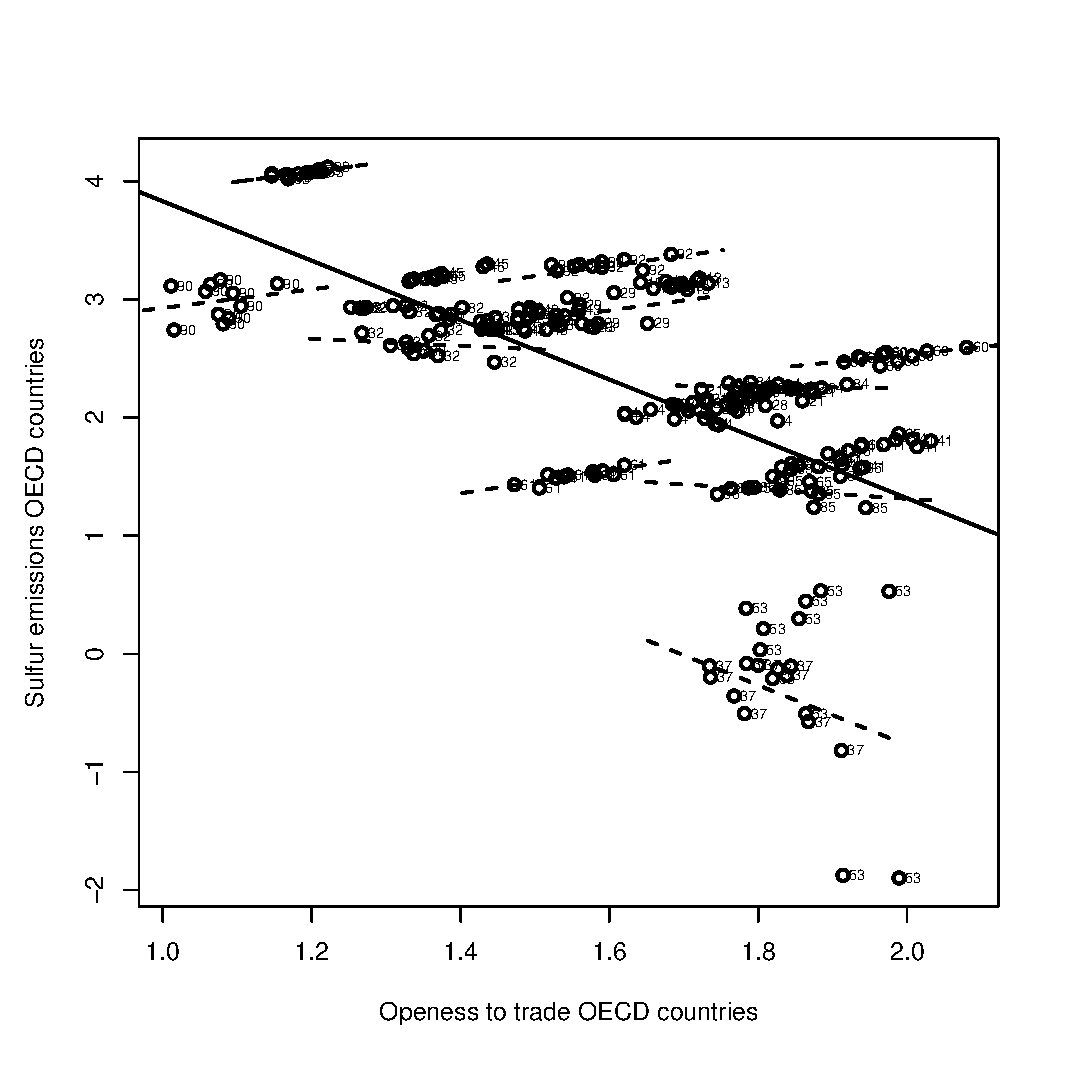
\includegraphics[angle=0,width=3.5in]{aee_hetero.ps}
%\end{figure}
%\end{center}
%
%The following regression output shows how including individual effects changes the results of the regression.
%
%\begin{verbatim}
%--> SAMPLE; all$
%--> REJECT; oe = 0 $
%--> REGRESS; lhs=Y
%    ;rhs= ltrade
%    ;Str=idx
%    ;period=Tit
%    ;output=0
%    ;?Fixed
%    ;Panel$
%
%+-----------------------------------------------------------------------+
%| OLS Without Group Dummy Variables                                     |
%| Ordinary    least squares regression    Weighting variable = none     |
%| Dep. var. = LSO      Mean=   2.264707042    , S.D.=   1.061961505     |
%| Model size: Observations =     231, Parameters =   2, Deg.Fr.=    229 |
%| Residuals:  Sum of squares= 164.6389021    , Std.Dev.=         .84791 |
%| Fit:        R-squared=  .365273, Adjusted R-squared =          .36250 |
%| Model test: F[  1,    229] =  131.78,    Prob value =          .00000 |
%| Diagnostic: Log-L =   -288.6592, Restricted(b=0) Log-L =    -341.1609 |
%|             LogAmemiyaPrCrt.=    -.321, Akaike Info. Crt.=      2.517 |
%| Panel Data Analysis of LSO        [ONE way]                           |
%|           Unconditional ANOVA (No regressors)                         |
%| Source      Variation        Deg. Free.     Mean Square               |
%| Between       249.613               20.         12.4807               |
%| Residual      9.77228              210.         .465347E-01           |
%| Total         259.385              230.         1.12776               |
%+-----------------------------------------------------------------------+
%+---------+--------------+----------------+--------+---------+----------+
%|Variable | Coefficient  | Standard Error |t-ratio |P[|T|>t] | Mean of X|
%+---------+--------------+----------------+--------+---------+----------+
% LTRADE   -2.513419689      .21894353      -11.480   .0000  1.6228419
% Constant  6.343589841      .35966379       17.638   .0000
%
%
%
%+-----------------------------------------------------------------------+
%| Least Squares with Group Dummy Variables                              |
%| Ordinary    least squares regression    Weighting variable = none     |
%| Dep. var. = LSO      Mean=   2.264707042    , S.D.=   1.061961505     |
%| Model size: Observations =     231, Parameters =  22, Deg.Fr.=    209 |
%| Residuals:  Sum of squares= 9.719877869    , Std.Dev.=         .21565 |
%| Fit:        R-squared=  .962527, Adjusted R-squared =          .95876 |
%| Model test: F[ 21,    209] =  255.64,    Prob value =          .00000 |
%| Diagnostic: Log-L =     38.1575, Restricted(b=0) Log-L =    -341.1609 |
%|             LogAmemiyaPrCrt.=   -2.977, Akaike Info. Crt.=      -.140 |
%| Estd. Autocorrelation of e(i,t)     .637004                           |
%+-----------------------------------------------------------------------+
%+---------+--------------+----------------+--------+---------+----------+
%|Variable | Coefficient  | Standard Error |t-ratio |P[|T|>t] | Mean of X|
%+---------+--------------+----------------+--------+---------+----------+
% LTRADE   -.3050596377      .28739261       -1.061   .2896  1.6228419
%\end{verbatim}

\newpage
\section{General Form of Panel Model}

\begin{itemize}
\item The \cbox{general form} of the panel data model used in this study is given by the equation

%
%The specification used, using the variable  defined
%in Section \ref{sec:data}, is
%

\begin{equation}\label{eq:modd}
Y_{it} = \mu +    
\sum_{j= 1}^{k} \beta_{j} \; {X_{j}}_{it} + u_{\scriptscriptstyle{it}},
\end{equation}
with \(i=1, \ldots, N\) and \( t= 1, \ldots, T_i\) representing
groups and types respectively.
%Here  \(Y_{it}\) is a measure of pollution emissions, \({X_{0}}_{it}\)  is  income,\linelabel{lin:income}
%and \({X_{j}}_{it}\), for \(j=1, \dots, k-p\), denote the other socio-demographic control variables
%from the ACORN database that correspond to  additional determinants of  emissions. \(p\) is the order
%of the polynomial in income,
\(k\) the total number of regressors.

%variables consists of control variables that
%correspond to  additional determinants of environmental quality
%proposed by researchers.
%with \(i=1, \ldots, N\) and \( t= 1, \ldots, T_i\) representing
%groups and types respectively. The unobserved group specific effects
%are denoted by \(u_i\) in Equation~\ref{eq:modd}.
%
\item The \cbox{error component}, \(u_{it}\), in Equation~\ref{eq:modd}, can take different structures.
\item  The specification of
error components can depend solely on the contry/individual, \cbox{one-way} error component,  to which the observation
belongs or both on the country and year, \cbox{two-way} error component. 
%\begin{itemize}
\item If the specification depends on
country/individual, then we have \(u_{it} =  \alpha_i + \epsilon_{it}\).
The term \(\alpha_i\) is intended to capture the heterogeneity across
countries and \(\epsilon_{it}\) is the classical error term with
zero mean and a constant variance. 
\item Moreover, the individual effects, \(\alpha_i\),
can be assumed to be either \emph{fixed} or \emph{random}. 
\begin{itemize}
\item
If assumed \cbox{fixed}, the
\(\alpha_i\)s can be estimated by including a dummy variable for each country $i$,% i.e.,
%by replacing \(\mu\) with  the terms $\sum_{j=1}^N \alpha_i d_{ij}$, where $d_{ij} = 1$ if $i=j$ and 0 otherwise.
The $N$ \(\alpha_i\)s can then be estimated by ordinary least squares 
%complemented with suitably adjusted covariance matrix.\footnote{This is known as
%the least squares dummy variable (LSVD) estimator.}
\item  If  \cbox{random} the \(\alpha_i\)s  are assumed to be  IID with mean zero
and homoskedastic covariance matrix, \(\sigma_\alpha\), and  independent of the \(\epsilon_{it}\). 
\end{itemize}
\item 
The nature of the error structures
leads to different estimation procedures depending on the specification.
The latter assumptions will be tested in order to select the appropriate model.
%For this
%study, we estimated the models using ordinary least squares (OLS),  fixed effects (FE), and  random
%effects (RE),  with suitable specification  tests used to evaluate the appropriateness of
%each estimator.
For further details  on panel methods see
Verbeek (2008) or  Greene (2008).

\end{itemize}

\newpage
\subsection{Unobserved Individual--Specific Effects}
Panel methods allow to account for the effects of any combination of
omitted variables that remain constant over time.
The general model we are interested in estimating is a single equation
with individual effects of the form

\begin{equation}\label{eq:modd}
Y_{it} = \mu +
\sum_{j= 1}^{K} \beta_{j} \; {X_{j}}_{it} + \underbrace{\alpha_i +\epsilon_{it}}_{\text{one-way\\ error component} },
\end{equation}
%
%\begin{equation}\label{eq:indeff}
%y_{it} =  \alpha_i +  \beta_1 \; x_{it1} + \dots+ \beta_K \; x_{itK}   +\epsilon_{it}
%\end{equation}
%
with \(i=1, \ldots, N, \; t= 1, \ldots, T_i\).
\begin{enumerate}
\item ${X_{1}}_{it}, \ldots, {X_{K}}_{it}$ are \(K\) regressors (independent variables).
\item The \(\alpha_i\)
capture the effects of those variables that are specific to the i\emph{th} individual
and that are constant over time (time invariant).
\item \(\epsilon_{it} \sim IID(0,\sigma^2_\epsilon) \).
% is independently and identically
%distributed over individuals and time with mean 0 and variance \(\sigma_\epsilon^2\).
\item  For \emph{balanced panels} \(T_i=T\). To keep notation simple we will
 assume that the panels we consider  are balanced.
\end{enumerate}

There are two main approaches to estimate models like (\ref{eq:indeff}), the \emph{fixed effects model} (FEM)  and the
\emph{random effects model} (REM).

\newpage
\subsubsection{Fixed Effects Model}
In the fixed effects model the individual-specific dummies are treated as \cbox{fixed constants}.
A practical implementation of the fixed effects model is by augmenting the standard regression model with
dummy variables
\begin{equation}
y_{it} = \alpha_1 D_{1it} + \alpha_2 D_{2it} + \cdots+  \beta_1 \; x_{it1} + \dots+ \beta_K \; x_{itK}  +\epsilon_{it}
\end{equation}
where \(D_{jit}\) is an \cbox{individual-specific dummy} variable
defined as
\[
D_{jit} =
\begin{cases}
    1, &\text{if $i=j$ }; \\
    0, &\text{otherwise}.
\end{cases}
\]
\begin{itemize}
\item Note that there is no general intercept \(\alpha\) in the model to
avoid the dummy variable trap.
\item This  estimator for the \(\beta\)'s goes under the name of \cbox{LSDV}, \textbf{Least  Squares  with
Dummy Variables},  estimator.
\item This model can be estimated by \cbox{OLS} after creating \(N\), \(D_i\) dummies.
\item A computationally \cbox{simpler} approach consists of regressing (\(y_{it} - y_{i.}\)) on
(\(x_{it} - x_{i.}\)), using OLS with no constant, where
\(y_{i.}\) is the individual-specific mean of \(y\) and \(x_{i.}\) are the \(N\)
individual-specific means of \(x_{it}\).
\item The transformation that produces observations in \textbf{deviations from individual means}
is called the \cbox{\emph{within}} transformation.
\item The individual-specific intercepts are recovered by calculating
\(\widehat{\alpha}_i = y_{i.} -x_{i.1} \widehat{\beta}^{FE}_{1} - \cdots -x_{i.K} \widehat{\beta}^{FE}_{K}\).
\end{itemize}
\newpage
\subsubsection{Random Effects Model}
If  random the \(\alpha_i\)s  are assumed to be  IID with mean zero
and homoskedastic covariance matrix, \(\sigma_\alpha\), and  independent of the \(\epsilon_{it}\). 
The REM can be represented by the equation
\begin{equation}\label{eq:rem}
y_{it} =  \mu +  \beta_1 \; x_{it1} + \dots+ \beta_K \; x_{itK} + \alpha_i  +\epsilon_{it}
\end{equation}
with
\begin{enumerate}
\item \(E[\alpha_{i}] = 0\); \(\var[\alpha_{i}]= \sigma^2_\alpha\).
\item \(\cov[\epsilon_{it},\alpha_i]=0\).
\item \(\var[\epsilon_{it}+\alpha_{i}] = \sigma^2 = \sigma^2_\epsilon + \sigma^2_\alpha\).
\item \(\corr[ \epsilon_{it} +\alpha_i ,\epsilon_{is} +\alpha_i]=\rho=\frac{\sigma^2_u}{\sigma^2},
 \qquad \text{for $s \neq t$}.  \)
\end{enumerate}
\begin{itemize}
\item
Equation~\ref{eq:rem} includes a general intercept \(\alpha\). The dummy variable trap is avoided
by assuming that the the expectation individual-specific errors, \(\alpha_i\), is zero.
\item The individual-specific effect is now represented as a stochastic component  \(\alpha_i\), of the same type
as the error term \(\epsilon_{it}\).
\item The REM requires is estimated by GLS (Generalized Least Squares). Basically, the estimation involves using OLS
to regress \((y_{it} - \theta y_{i.})\) on (\(1-\theta\)) and \((x_{it} - \theta x_{i.})\)
where (\(1-\theta\)) corresponds to the constant term. The GLS estimate  of the REM model
is equivalent to applying the OLS method to the original data transformed by removing a fraction \(\theta\)
of the individual-specific means, \(y_{i.}\) and \(x_{i.}\) (instead of the whole means as with the within transformation).
\item \(\theta\) is calculated as  \(1 - \vartheta\)
where \(\vartheta = \frac{\sigma_\epsilon^2}{\sigma_\epsilon^2 + T \sigma_\alpha^2}\).
\end{itemize}
\newpage
\subsection{Unobserved Time--Specific Effects}
In many cases we would like to include time-specific effects in our models
\[
Y_{it} = \mu +
\sum_{j= 1}^{K} \beta_{j} \; {X_{j}}_{it}  +  \underbrace{\alpha_i + \lambda_t +\epsilon_{it}}_{\text{two-way error component} }
\]
with \(i=1, \ldots, N, \; t= 1, \ldots, T_i\) and where \(\alpha_i\) and \(\lambda_t\) are
respectively individual and time specific effects.
\newpage
\subsection{Unobserved Time and Individual--Varying Effects}
If no candidate variable such as openness to trade is available, we might have to resort to
lagged dependent variables.
\[
y_{it} =\gamma_1  y_{i(t-1)} + \beta_1 \; x_{it1} + \dots+ \beta_k \; x_{itk} + \lambda_{t} +  \alpha_i +\epsilon_{it}
\]
with \(i=1, \ldots, N, \; t= q+1, \ldots, T_i\), where \(\alpha_i\) and \(\lambda_t\) are
respectively individual and time specific effects.

\newpage

%\section{Panel Data Models Estimation}
\subsection{First difference (FD) Estimator}
One approach to account for individual heterogeneity is simply to get rid of it by first differencing.
\begin{equation}\label{eq:curr}
y_{it} =  \beta \; x_{it}  +  \alpha_i +\epsilon_{it}
\end{equation}

\begin{equation}\label{eq:lag}
y_{i(t-1)} =  \beta \; x_{i(t-1)}  +  \alpha_i + \epsilon_{i(t-1)}
\end{equation}

Subtracting (\ref{eq:lag}) from (\ref{eq:curr}), we get

\begin{equation*}\label{eq:diff}
y_{it} - y_{i(t-1)} =  \beta ( \; x_{it}-  x_{i(t-1)})  + (\epsilon_{it} - \epsilon_{i(t-1)})
\end{equation*}

\begin{equation}\label{eq:diff2}
\Delta y_{it} =  \beta \Delta x_{it}  + \Delta \epsilon_{it}
\end{equation}
Assuming that \(\Delta \epsilon_{it}\) are uncorrelated with  \(\Delta x_{it1}\), we can estimate (\ref{eq:diff2}) by OLS.
This is called that first-differenced estimator.
%\subsection{Fixed and Random Effects Estimators}
%%Want to attribute variability in the data to various categorization of the data.
%%
%%
%%We classify data in terms of factors and their levels. We want to know the extent to which
%%different levels of a factor affect the variable of interest.
%%
%%The effect of a factor are of two kinds: fixed and random.
%
%\subsection{Fixed Effects (FE)}
%
%%Fixed effects are the effects attributable to a finite set of levels of a factor that occur in the data
%\begin{itemize}
%
%\item Suppose per capita emissions in 20 different countries
%are investigated.
%
%\item If for country \(i\) we
%have \(T\) measurements of per capita emissions and the level of
%per capita emissions for country \(i\) in time \(t\) is \(y_{it}\)
%then a possible model would be, if we want to know the individual
%effect on pollution of the countries considered,
%
%\[E[y_{it}] = \mu_i\]
%
%where \(E\)  represents expectation and \(\mu_i\) is the expected per capita emission
%in country \(i\). We can write \(\mu_i = \mu + \alpha_i\) and therefore have
%
%\[E[y_{it}] = \mu + \alpha_i\]
%
%
%\item In this modeling of the expected value of \(y_{ij} \) each \(\alpha_i\)
%is considered a fixed unknown constant, the magnitude of which is of interest to us.
%
%\item We focus only on the countries included in the sample, and no other.
%For this reason the effects are called fixed effects.
%\end{itemize}
%%\newpage
%\subsection{Random Effects (RE)}
%%
%%Random effects are attributable to a infinite set of levels of a
%%factor, of which only a random sample are deemed to occur in the data.
%%
%%
%Again considering per capita emissions in the 20 different
%countries. It is not unreasonable to think of these countries as a
%randomly chosen sample of countries from a population of
%countries. If for country \(i\) we have \(T\) measurements of per
%capita emissions and the level of per capita emissions for country
%\(i\) at time \(t\) is \(y_{it}\) then a possible model would be
%
%\[E[y_{it}] = \mu + \alpha_i\]
%\begin{itemize}
%\item Although this model is algebraically the same as the previous one, some underlying assumptions
%are different. In the previous case \(\alpha_i\)  is a fixed effect, the effect on pollution
%of a chosen country \(i\). But in the latter model \(\alpha_i\) is the effect on pollution
%in the observed country \(i\) which is viewed as just one country, one randomly chosen from a  population.
%\item The country labeled \(i\) is of no interest by itself. This is the main characteristics of
%the random effects, the fact that they can be used as the basis for making inferences
%about the population from which they have come from.
%
%\item With the \(\alpha_i\) being treated as random variables, we must assign a distribution to them.
%Usually it is assumed that all \(\alpha_i\)'s are independently and identically distributed with mean 0 and
%same variance \(\sigma^2_\alpha\)
%\end{itemize}

\newpage
\section{Model Specification}

\subsection{ OLS Vs. Individual Effects}
The (Breusch and Pagan) LM-test is used to test the hypothesis that individual effects are significant.
 If these tests do not provide any evidence for individual effects,
 then the model can simply be estimated by ordinary least squares (OLS).
A large value of the LM statistic argues in favor of the of a panel data model

\newpage
\subsection{Fixed Vs. Random Effects}
\begin{itemize}
    \item The estimated parameters can differ quite substantially if \emph{T} is small and \emph{N} large.
    \item So if the number of individual, say countries, is small and we are interested in the \(\alpha_i\),
    it makes sense to prefer the FE estimator.
    \item With large population, if interested in making inference about the population, the RE estimator might
    be more appropriate.
    \item Even in the case of a large population of individual countries, we might still opt for the FE estimator.
    \begin{itemize}
        \item If the individual effects, \(\alpha_i\), are correlated with the regressors. In this case
        the RE estimator is inconsistent.
        \item  The Hausman test is used to decide whether the regressors are correlated with the
    individual effect.
    A small Hausman statistic argues in favor of the random effect model, a large in favor of a fixed effects one.
   \end{itemize}
   Sometimes, the RE might be preferable, even when the individual effects are correlated with
   the regressors.
    \begin{itemize}
    \item The FE estimator allows \(\alpha_i\) and \(x_{it}\) to be arbitrarily correlated by
        eliminating, as in the FD estimator, the individual effects and all time-invariant effects.
        We cannot therefore include in our model variables that are constant over time, e.g., in the EKC example,
        OECD/non OECD dummy.
    \end{itemize}
\end{itemize}



%vspace{1cm}
%\subsection{\begin{pspicture}(0,0)(3,1.4)
%  \psset{linecolor=white}
%  \pstextpath{\pscurve
%( 0.0000000 ,0.0000000)
%( 0.0000000 ,0.0000000)
%( 0.3333333 ,0.5925926)
%( 0.6666667 ,1.0370370)
%( 1.0000000 ,1.3333333)
%( 1.3333333 ,1.4814815)
%( 1.6666667 ,1.4814815)
%( 2.0000000 ,1.3333333)
%( 2.3333333 ,1.0370370)
%( 2.6666667 ,0.5925926)
%( 3.0000000 ,0.0000000)
%( 3.0000000 ,0.0000000)} {\color{black}  EKC Computations}
%\end{pspicture}}

\newpage
\section{Reading Data}
\begin{CVerbatim}
stern.dat <- read.table("e:/jan/stern2.dat",header=T)
attach(stern.dat)

> names(stern.dat)
[1] "year"    "country" "pop"     "so"      "gdppc"   "sopc"    "oe"

> head(stern.dat)
  year country   pop      so gdppc    sopc oe
1 1960      54 17910 1099.72  7258 0.06140  1
2 1961      54 18270 1076.06  7261 0.05890  1
3 1962      54 18614 1073.68  7605 0.05768  1
4 1963      54 18963 1087.53  7876 0.05735  1
5 1964      54 19326 1142.22  8244 0.05910  1
6 1965      54 19678 1206.56  8664 0.06132  1

\end{CVerbatim}
%? For my system
%READ; file=F:\web\statmeth\stern.dat; nvar=7; nobs=2294
%   ; names=year, country, pop, so, gdpc, sopc, oe$
%CREATE ; lgdp = log(gdpc)
%       ; lgdpsq=lgdp*lgdp
%       ; lsopc=log(sopc)$
%CREATE  ;  Time  =  Trn(-31,0) $
%? or
%CREATE  ; Tt = year - 1959 $
%REGRESS  ;Lhs=lsopc
%         ;Rhs=lgdp,lgdpsq
%         ;Str=country
%         ;period=Time
%         ;Output=2
%         ;Panel$
%
%\verb"
\newpage
\section{Descriptive Statistics}

We  can now summarise the data in many ways.
%
%\begin{CVerbatim}
%DSTAT; Rhs=pop, so, gdpc, sopc, oe$
%\end{CVerbatim}
%
\begin{CVerbatim}
> summary(stern.dat)
      year         country            pop                so               gdppc
 Min.   :1960   Min.   :  1.00   Min.   :    231   Min.   :    0.01   Min.   :  303
 1st Qu.:1967   1st Qu.: 62.00   1st Qu.:   5063   1st Qu.:   14.67   1st Qu.: 1548
 Median :1975   Median : 94.50   Median :  12764   Median :  101.22   Median : 3566
 Mean   :1975   Mean   : 90.69   Mean   :  47466   Mean   :  703.03   Mean   : 5360
 3rd Qu.:1983   3rd Qu.:123.00   3rd Qu.:  32979   3rd Qu.:  448.50   3rd Qu.: 7728
 Max.   :1990   Max.   :147.00   Max.   :1133683   Max.   :14213.89   Max.   :80831
      sopc                 oe
 Min.   :8.900e-07   Min.   :0.0000
 1st Qu.:1.960e-03   1st Qu.:0.0000
 Median :9.673e-03   Median :0.0000
 Mean   :2.150e-02   Mean   :0.3108
 3rd Qu.:2.780e-02   3rd Qu.:1.0000
 Max.   :4.656e-01   Max.   :1.0000
\end{CVerbatim}
\newpage
\begin{CVerbatim}
  aggregate(stern.dat, by = list( oe ),  FUN= "mean" )
  Group.1 year   country      pop        so    gdppc       sopc oe
1       0 1975  75.58824 54261.85  545.0277 3614.351 0.02061154  0
2       1 1975 124.17391 32397.30 1053.3722 9230.491 0.02347759  1

\end{CVerbatim}
%

%\newpage
\section{Creating and Transforming Variables}
For the whole sample create squared and log terms.
\begin{CVerbatim}
lso <- log(sopc)
lgdp <- log(gdppc)
lgdp2 <- lgdp^2
\end{CVerbatim}



\section{Plotting Data}
\begin{CVerbatim}
plot(lgdp,lso)
\end{CVerbatim}
The resultiong LimDep plot is shown in
figure~\ref{fig:aee_progroup}.

\begin{figure}
  \begin{center}
    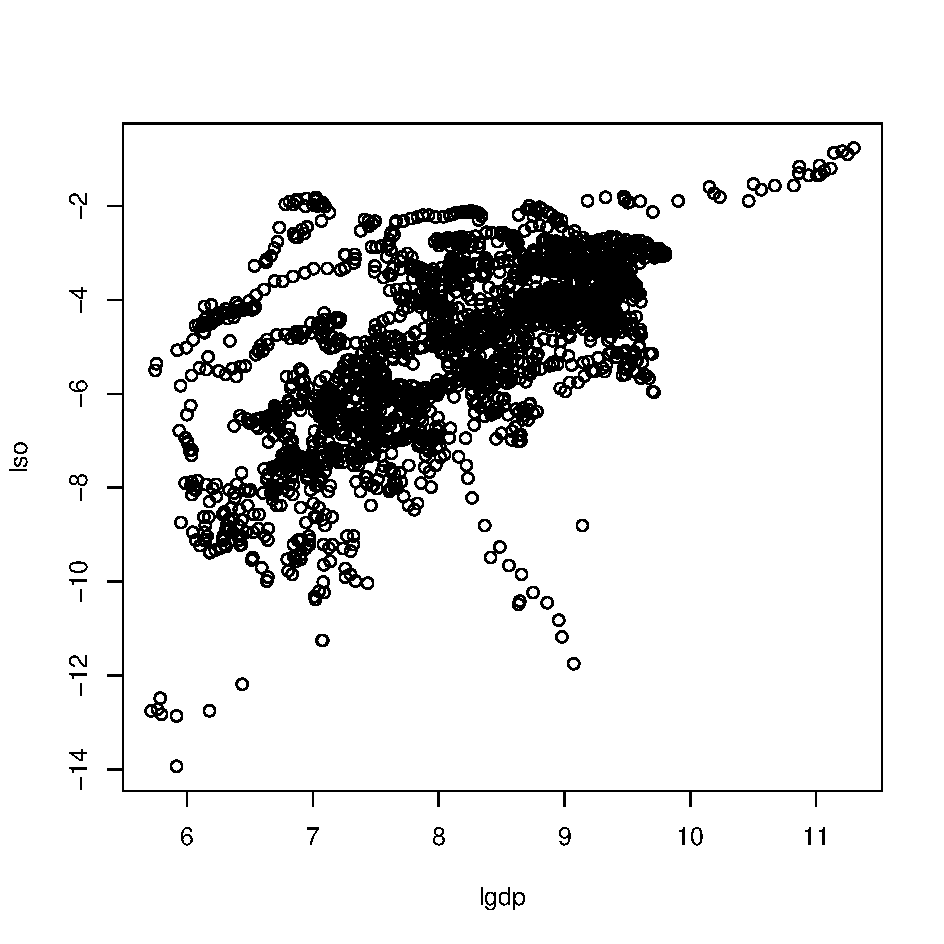
\includegraphics[width=6.5in]{aee_panel_exer_limall.pdf}
  \end{center}
  \caption{R plot \label{fig:aee_progroup}}
\end{figure}

%\newpage
\clearpage
\section{Running Panel Regressions in R}
\begin{CVerbatim}
library(plm)

stern.fra <- data.frame(
    cbind(
    country = country,
    year=year,
    oe=oe,
    lso = log(sopc),
    lgdp = log(gdppc),
    lgdp2 = lgdp^2
    )
)

stern.plm <- plm.data(stern.fra, index = c("country","year"))

\end{CVerbatim}
\newpage
%The output is divided into four parts.
%\begin{enumerate}
%    \item The first part gives the OLS (OLS Without Group Dummy Variables)
%estimates,
%    \item the second the fixed effect estimates (Least Squares with Group Dummy Variables),
%    \item the third the random effect estimates, and
%    \item the fourth the fixed individuals and time effects estimates.
%\end{enumerate}
%Note that:
%\begin{itemize}
%\item you can suppress one of the panel models this is useful to compute turning points of a specific model)
% by including the subcommands \textbf{; Fixed} or \textbf{; Random}
%\item it is not necessary to include \textbf{ONE} amongst the regressors
%\item to obtain a list of the fixed effects use the \textbf{;Output = 2} subcommand
%\end{itemize}
%
%To obtain the estimates of the FE model  or just the RE (this is useful to compute turning points of a specific model),
%the subcommands \textbf{; Fixed} and
%\textbf{; Random}, can be added.
\newpage
\subsection{OLS}
\begin{CVerbatim}
> stern.ols <- plm(lso ~ lgdp  + lgdp2, data=stern.plm, \fbox{\textcolor{red}{model = "pooling"}})
> summary(stern.ols)
Oneway (individual) effect Pooling Model

Call:
plm(formula = lso ~ lgdp + lgdp2, data = stern.plm, model = "pooling")

Balanced Panel: n=74, T=31, N=2294

Residuals :
    Min.  1st Qu.   Median  3rd Qu.     Max.
-7.80000 -0.85100 -0.00892  0.83200  4.65000

Coefficients :
            Estimate Std. Error t-value Pr(>|t|)
(Intercept) -17.0282     1.7525   -9.72  < 2e-16 ***
lgdp          1.8209     0.4380    4.16  3.3e-05 ***
lgdp2        -0.0418     0.0271   -1.54     0.12
---
Signif. codes:  0 ?***? 0.001 ?**? 0.01 ?*? 0.05 ?.? 0.1 ? ? 1

Total Sum of Squares:    8110
Residual Sum of Squares: 5090
F-statistic: 679.914 on 2 and 2291 DF, p-value: <2e-16

\end{CVerbatim}


\newpage
\subsection{Fixed (within) Individual Country Effects}
\begin{CVerbatim}
> stern.fe <- plm( lso ~ lgdp  + lgdp2, data=stern.plm,  
   model = \fbox{\textcolor{red}{"within"}}, effect = \fbox{\textcolor{red}{"individual"}})
> summary(stern.fe)
Oneway (individual) effect Within Model

Call:
plm(formula = lso ~ lgdp + lgdp2, data = stern.plm, effect = "individual",
    model = "within")

Balanced Panel: n=74, T=31, N=2294

Residuals :
   Min. 1st Qu.  Median 3rd Qu.    Max.
-4.3300 -0.1860  0.0291  0.2360  3.2900

Coefficients :
      Estimate Std. Error t-value Pr(>|t|)
lgdp    3.2528     0.3533    9.21  < 2e-16 ***
lgdp2  -0.1525     0.0213   -7.16  1.1e-12 ***
---
Signif. codes:  0 ?***? 0.001 ?**? 0.01 ?*? 0.05 ?.? 0.1 ? ? 1

Total Sum of Squares:    888
Residual Sum of Squares: 756
F-statistic: 192.867 on 2 and 2218 DF, p-value: <2e-16
\end{CVerbatim}

\newpage
\subsection{Accessing Fixed Country Individual Effects}
The estimated individual effects can be retrieved using the command \emph{fixef( stern.fe )}. The option 
\emph{dmean} produces differences from the mean. This is useful to contrast the fixed effects later with the
random effects.
\begin{CVerbatim}

> summary(\textcolor{red}{fixef}(stern.fe,effect ="individual",type = 'dmean'))
     Estimate Std. Error t-value Pr(>|t|)
1   -2.229050   1.475348 -1.5109  0.13082
14  -0.231877   1.454547 -0.1594  0.87334
18  -1.578418   1.432819 -1.1016  0.27063
22  -0.765428   1.421201 -0.5386  0.59018
25  -2.618924   1.436167 -1.8236  0.06822 .
\end{CVerbatim}

To produce a histogram of the fixed effects:
\begin{CVerbatim}
hist(fixef(stern.fe,effect ="individual",type = 'dmean'))
\end{CVerbatim}
\begin{center}
\begin{figure}[h!]
%\caption{Boundary bias of NW estimator\label{fig:ekcbiasbou0}}
%   \vspace{.1in}
  \centering \leavevmode 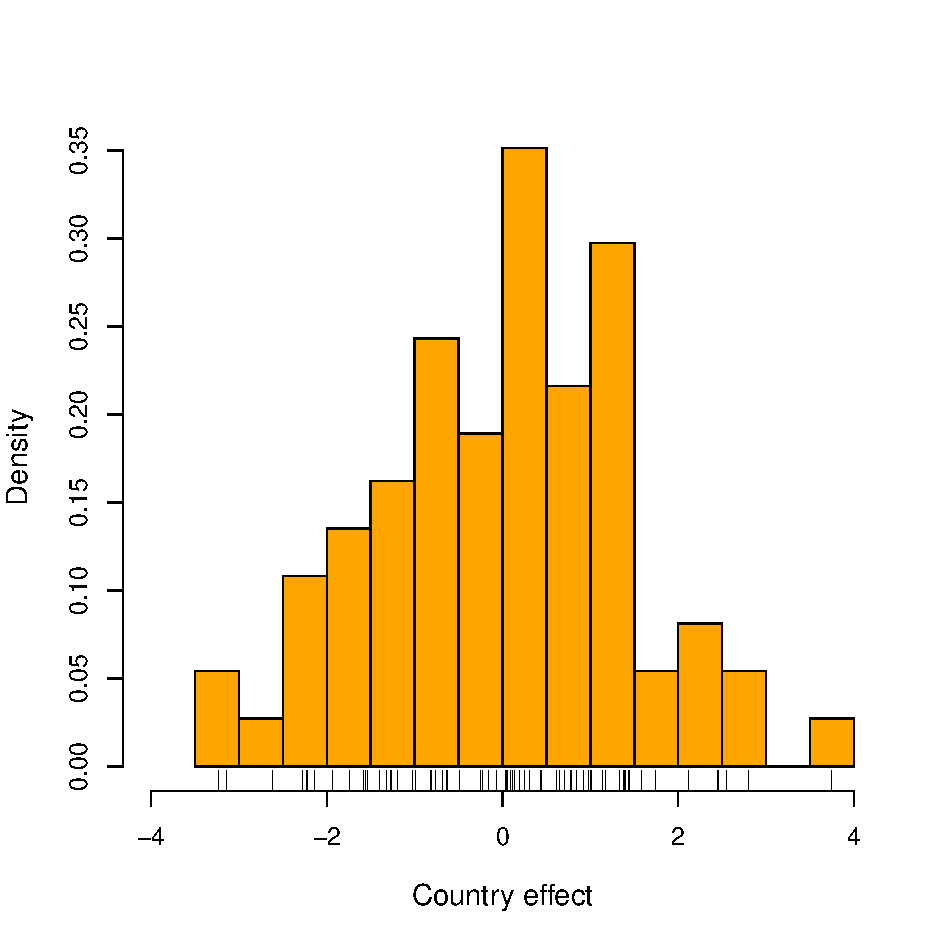
\includegraphics[angle=0,width=5.5in]{fixedcountryeff.pdf}
  % \parbox{5in}{ \caption{\footnotesize Time Effects for World Plus or Minus Two sd. }\label{fig:aee_panel_exer_teall}}
\end{figure}
\end{center}

\clearpage
\newpage
\subsection{Random Country Individual Effects}
\begin{CVerbatim}
> stern.re <- plm( lso ~ lgdp  + lgdp2, 
           data=stern.plm,  \fbox{\textcolor{red}{model="random"}}, \fbox{\textcolor{red}{effect = "individual"}})
> summary(stern.re)
Oneway (individual) effect Random Effect Model
   (Swamy-Arora's transformation)

Call:
plm(formula = lso ~ lgdp + lgdp2, data = stern.plm, effect = "individual",
    model = "random")

Balanced Panel: n=74, T=31, N=2294

\textcolor{red}{Effects:}
                var std.dev share
idiosyncratic 0.341   0.584  0.15
\textcolor{red}{individual}    1.934   \fbox{\textcolor{red}{1.391}}  0.85
theta:  0.925

Residuals :
   Min. 1st Qu.  Median 3rd Qu.    Max.
-4.5700 -0.1680  0.0551  0.2520  3.0400

Coefficients :
            Estimate Std. Error t-value Pr(>|t|)
(Intercept) -21.3789     1.4538  -14.71  < 2e-16 ***
lgdp          3.2663     0.3498    9.34  < 2e-16 ***
lgdp2        -0.1521     0.0211   -7.20  7.9e-13 ***
---
Signif. codes:  0 ?***? 0.001 ?**? 0.01 ?*? 0.05 ?.? 0.1 ? ? 1

Total Sum of Squares:    928
Residual Sum of Squares: 782
F-statistic: 213.906 on 2 and 2291 DF, p-value: <2e-16
\end{CVerbatim}

\newpage
\clearpage
\subsection{Fixed vs Random Country Effects}
We can plot:
\begin{enumerate}
\item 
 a histogram of the fixed effects:
\begin{CVerbatim}
fief <- fixef(stern.fe,effect ="individual",type = 'dmean')

\textcolor{red}{hist}( fief, freq=F, br=20, xlab="Country effect",main="",col="orange")
\end{CVerbatim}
\item A reference normal
\begin{CVerbatim}
 curve(\textcolor{red}{dnorm}(x,sd=1.3906),add=T,lty=3,lwd=2)
\end{CVerbatim}
\item An a nonparametric Kernel estimator:
\begin{CVerbatim}
lines(\textcolor{red}{density}( fief ),col="red")
\end{CVerbatim}
\end{enumerate}
\begin{center}
\begin{figure}[h!]
%\caption{Boundary bias of NW estimator\label{fig:ekcbiasbou0}}
%   \vspace{.1in}
  \centering \leavevmode 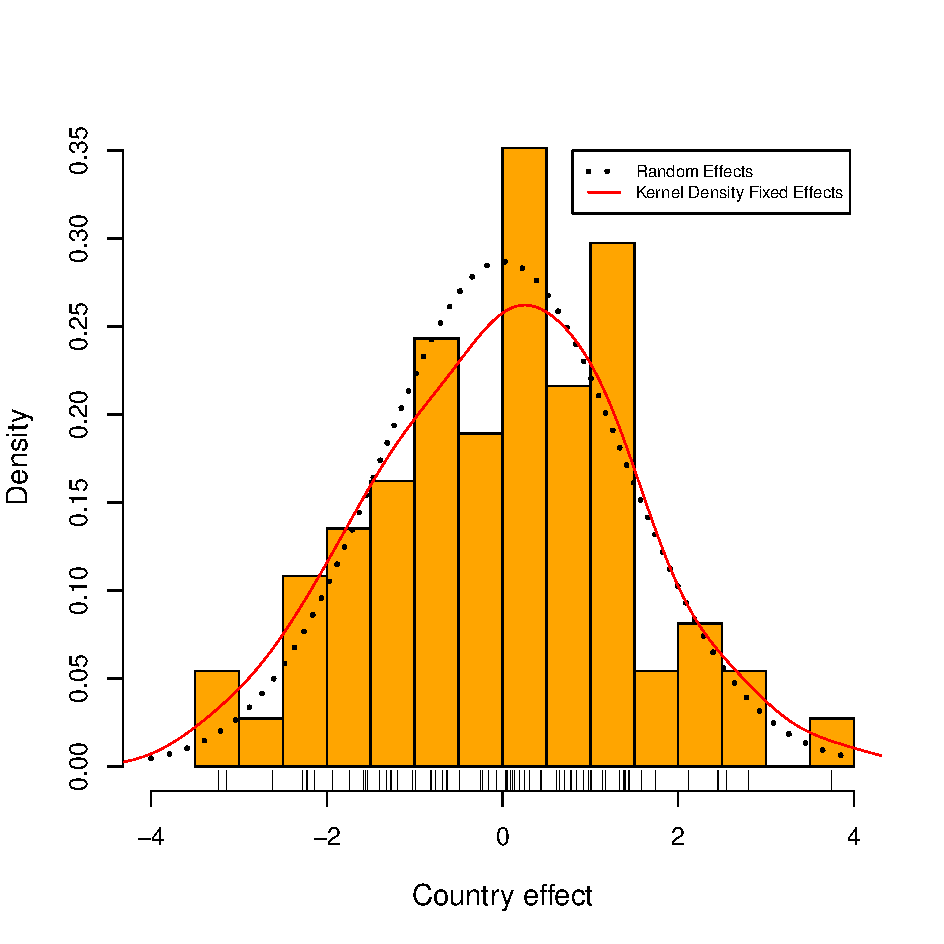
\includegraphics[angle=0,width=5.5in]{covsraeff.pdf}
  % \parbox{5in}{ \caption{\footnotesize Time Effects for World Plus or Minus Two sd. }\label{fig:aee_panel_exer_teall}}
\end{figure}
\end{center}

\newpage
\clearpage

\subsection{Fixed Country and Time Effects}
%Unlike the individual stratification dummy variable, the time dummy variable
%must be a sequence of integers starting at 1,  \( (1,2,\ldots, T)\).
%As noted earlier, it is not necessary for every group to have data in every period; there may be gaps.
%With a balanced  panel, it is possible to create the needed sequence using the CREATE Trn function. Also,
%knowing the starting date, one can subtract the starting year minus one to obtain the sequence.
%In our case, having 31 years, starting in 1960,
\begin{CVerbatim}
> stern2.fe <- plm( lso ~ lgdp  + lgdp2, data=stern.plm,  
       model = "within", \fbox{\textcolor{red}{effect = "twoways"}})
> summary(stern2.fe)
Twoways effects Within Model

Call:
plm(formula = lso ~ lgdp + lgdp2, data = stern.plm, effect = "twoways",
    model = "within")

Balanced Panel: n=74, T=31, N=2294

Residuals :
   Min. 1st Qu.  Median 3rd Qu.    Max.
-4.4200 -0.1800  0.0209  0.2220  3.2700

Coefficients :
      Estimate Std. Error t-value Pr(>|t|)
lgdp    3.8465     0.3653   10.53  < 2e-16 ***
lgdp2  -0.1706     0.0215   -7.94  3.1e-15 ***
---
Signif. codes:  0 ?***? 0.001 ?**? 0.01 ?*? 0.05 ?.? 0.1 ? ? 1

Total Sum of Squares:    850
Residual Sum of Squares: 728
F-statistic: 182.654 on 2 and 2188 DF, p-value: <2e-16
\end{CVerbatim}
\newpage
\begin{CVerbatim}
> summary(fixef(stern2.fe,effect ="time"))
     Estimate Std. Error t-value  Pr(>|t|)
1960 -24.6897     1.5494 -15.935 < 2.2e-16 ***
1961 -24.6987     1.5500 -15.935 < 2.2e-16 ***
1962 -24.7813     1.5517 -15.971 < 2.2e-16 ***
1963 -24.6937     1.5530 -15.900 < 2.2e-16 ***
1964 -24.6841     1.5543 -15.881 < 2.2e-16 ***
1965 -24.6817     1.5556 -15.866 < 2.2e-16 ***
1966 -24.6537     1.5564 -15.840 < 2.2e-16 ***
1967 -24.6449     1.5571 -15.827 < 2.2e-16 ***
1968 -24.6933     1.5583 -15.846 < 2.2e-16 ***
1969 -24.7453     1.5602 -15.861 < 2.2e-16 ***
1970 -24.7014     1.5621 -15.813 < 2.2e-16 ***
1971 -24.7304     1.5637 -15.815 < 2.2e-16 ***
1972 -24.7821     1.5643 -15.842 < 2.2e-16 ***
...
\end{CVerbatim}
%
\newpage
%\begin{CVerbatim}
%summary(fixef(stern.fe,effect ="individual",type = 'dmean'))[,1]
%          1          14          18          22          25          30          31          32
%-2.22904982 -0.23187714 -1.57841758 -0.76542837 -2.61892398 -0.48527165 -1.27951557  1.58296386
%         34          41          44          46          48          49          50          52
%-3.22945670  1.42893499 -2.27496160 -1.53280802  2.45941549  3.74035664  1.14086645 -1.26157389
%         54          60          62          64          65          71          72          73
% 1.33168786 -2.14276590 -1.02213404  0.09306713 -0.99245493  1.44522191  1.17604885 -1.93332198
%         74          75          76          77          81          83          84          88
%-0.62627545 -0.82522209  2.11257052 -0.81133062  1.00389393 -0.99576723  0.78175232  1.37774436
%         89          90          91          92          94          95          97          98
%-3.13669312 -0.16399749 -1.74481298 -0.24772560  0.24859778  0.05726724  0.19887546  2.44842906
%        100         102         106         108         109         110         111         112
%-1.40505989 -0.63641969  0.03835032  0.97700926  1.39102170 -2.21917479 -1.19841019  0.25547058
%        113         116         117         119         120         121         122         123
%-1.56388005  0.11045294  0.91672646  0.42736985  2.79813956  0.44608478  0.61370754  0.24494193
%        125         126         129         130         131         133         134         136
% 0.84447285  0.77209870  0.30685759 -0.07359527 -0.67759197  0.70255390 -0.15995900 -0.62124387
%        137         138         139         140         141         142         143         144
% 2.55134203  0.13246764  0.04577610 -1.32296892  0.65304780  1.14378865  1.40300595  1.74700238
%        145         147
% 1.01654970 -0.15784268
% \end{CVerbatim}
% \newpage
\begin{CVerbatim}
fe.1 <- summary(fixef(stern2.fe,\fbox{\textcolor{red}{effect ="time"}}))[,1]
plot(1960:1990,fe.1,type="l",xlab="Year",ylab="Period effect",ylim=rang)
\end{CVerbatim}
\newpage
%Now the file \texttt{panelie.out} will contain the Time effects.
The following Figure 
shows the time effects.

\begin{center}
\begin{figure}[h!]
%\caption{Boundary bias of NW estimator\label{fig:ekcbiasbou0}}
%   \vspace{.1in}
  \centering \leavevmode 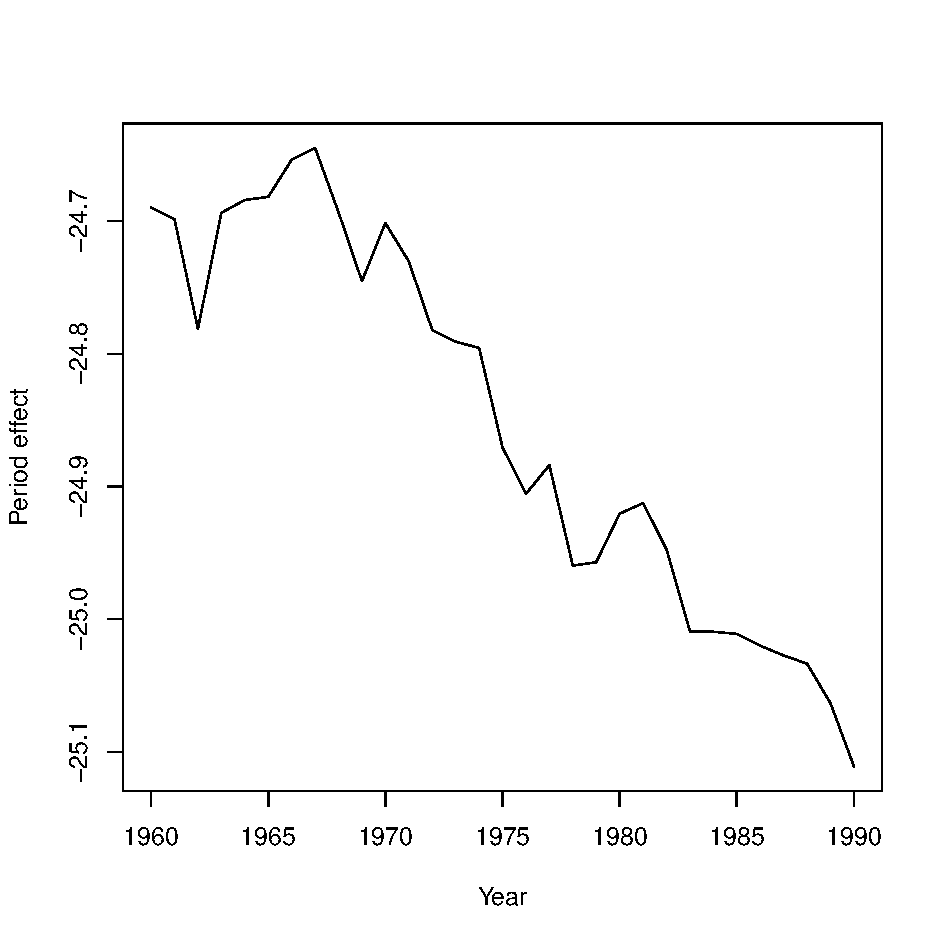
\includegraphics[angle=0,width=5.2in]{periodeffectr.pdf}
  % \parbox{5in}{ \caption{\footnotesize Time Effects for World Plus or Minus Two sd. }\label{fig:aee_panel_exer_teall}}
\end{figure}
\end{center}

\clearpage
\newpage
\subsection{First-differences Estimator}
%Unlike the individual stratification dummy variable, the time dummy variable
%must be a sequence of integers starting at 1,  \( (1,2,\ldots, T)\).
%As noted earlier, it is not necessary for every group to have data in every period; there may be gaps.
%With a balanced  panel, it is possible to create the needed sequence using the CREATE Trn function. Also,
%knowing the starting date, one can subtract the starting year minus one to obtain the sequence.
%In our case, having 31 years, starting in 1960,
\begin{CVerbatim}
> stern.fd <- plm( lso ~ lgdp  + lgdp2, 
      data=stern.plm,  \fbox{\textcolor{red}{model = "fd"}}, effect = "individual")
> summary(stern.fd)
Oneway (individual) effect First-Difference Model

Call:
plm(formula = lso ~ lgdp + lgdp2, data = stern.plm, effect = "individual",
    model = "fd")

Balanced Panel: n=74, T=31, N=2294

Residuals :
    Min.  1st Qu.   Median  3rd Qu.     Max.
-3.37000 -0.07210 -0.00618  0.05760  4.09000

Coefficients :
            Estimate Std. Error t-value Pr(>|t|)
(intercept) -0.00378    0.00623   -0.61   0.5442
lgdp         2.07434    0.73995    2.80   0.0051 **
lgdp2       -0.08990    0.04623   -1.94   0.0519 .
---
Signif. codes:  0 ?***? 0.001 ?**? 0.01 ?*? 0.05 ?.? 0.1 ? ? 1

Total Sum of Squares:    168
Residual Sum of Squares: 165
F-statistic: 22.3866 on 2 and 2217 DF, p-value: 2.37e-10
\end{CVerbatim}
%
\newpage
\section{Model specification: OLS Vs. Individual Effects, Fixed Vs. Random Effects}
\begin{itemize}
\item 
 First, the (Breusch and Pagan) \cbox{LM-test} is used to test \textbf{the hypothesis that individual effects are significant}.
 If these tests do not provide any evidence for individual effects,
 then the model can simply be estimated by ordinary least squares (OLS).

\item 
 Second, the \cbox{Hausman test} is used to decide whether the \textbf{regressors are correlated with the
 individual effect}.

\item 
The large value of the LM statistic argues in favor of the of a panel data model, the small Hausman
statistic argues in favor of the random effect model. A small Hausman
statistic argues in favor of the random effect model, a large in favor of a fixed effects one.
\end{itemize}
\newpage
\begin{itemize}
\item 
The \cbox{LM test} is based on the idea that if the variance
of the individual effects
is zero then the random effects model model reduces to the pooled OLS model.
\item The null  \cbox{hypothesis} tested is
 $$\mathbf{H}_0\!\!:  \sigma_\alpha^2 = 0$$
 \vspace{.1in}
\begin{CVerbatim}
> plmtest(  lso ~ lgdp  + lgdp2, data=stern.plm, type="bp", effect = c("twoways"))

        \fbox{\textcolor{red}{Lagrange Multiplier Test}} - two-ways effects (Breusch-Pagan)

data:  lso ~ lgdp + lgdp2
chisq = 24163, df = 2, p-value < 2.2e-16
alternative hypothesis: significant effects 
\end{CVerbatim}
\vspace{.1in}
\item The LM statistic is  24163 and assessed against the
\(\chi^2\) distribution with 2 degrees of freedom is  
significant at any conventional level level ($p$-value $\approx 0.00$).
\item We can conclude that country effects  are considerably important and that \cbox{panel methods} are
necessary to determine the impact of income factors on the emissions.
\end{itemize}
\newpage
\begin{itemize}
\item To decide between  fixed  and random effects approach to panel data estimation, we can
use the \cbox{Hausman} test (1978),
 \item The null  \cbox{hypothesis} tested is
$$\mathbf{H}_0\!\!:  \corr (\alpha_i, X_{i,t}) = 0$$
 that
 the regressors are correlated with the individual effect.
\item If the individual effects, \(\alpha_i\), are correlated with
the regressors  the RE estimator is inconsistent.
\item   A small Hausman statistic argues in favor of the random effect model, a large in favor of a fixed effects one.

\vspace{.1in}
\begin{CVerbatim}
> phtest( stern.fe, stern.re )

        \fbox{\textcolor{red}{Hausman Test}}

data:  lso ~ lgdp + lgdp2
chisq = 6.2707, df = 2, p-value = 0.04348
alternative hypothesis: one model is inconsistent
\end{CVerbatim}
\vspace{.1in}
\item 
 The Hausman statistic is 6.2707   which  assessed against the
\(\chi^2\) distribution with 2 degrees of freedom is significant at
the 5 per cent level ($p$-value 0.04348). 
\item The \cbox{fixed effect} model is the preferred
model.
\end{itemize}
\newpage
\section{Selecting a Subsample}
To select a subsample of observation 
(for example to compute the regression  only for OECD or for non-OECD countries)
 for example, to
include only the OECD sample, we can issue the following commands.
\vspace{.1in}
\begin{CVerbatim}
> summary(stern.fe.oe)
Oneway (individual) effect Within Model

Call:
plm(formula = lso ~ lgdp + lgdp2, data = stern.plm, 
   \fbox{\textcolor{red}{subset = oe == 1}}, effect = "individual", model = "within")

Balanced Panel: n=23, T=31, N=713

Residuals :
    Min.  1st Qu.   Median  3rd Qu.     Max.
-1.11000 -0.16000  0.00648  0.15000  0.96400

Coefficients :
      Estimate Std. Error t-value  Pr(>|t|)
lgdp  12.24450    0.73052  16.761 < 2.2e-16 ***
lgdp2 -0.67121    0.04124 -16.276 < 2.2e-16 ***
---
Signif. codes:  0 ?***? 0.001 ?**? 0.01 ?*? 0.05 ?.? 0.1 ? ? 1

Total Sum of Squares:    70.142
Residual Sum of Squares: 45.805
F-statistic: 182.773 on 2 and 688 DF, p-value: < 2.22e-16
\end{CVerbatim}

\newpage
\section{Other Tests}
Autocorrelation:
\begin{itemize}
\item  \cbox{Breusch-Godfrey test} for Panel models
\vspace{.1in}
\begin{CVerbatim}
library(lmtest)


pbgtest(stern.fe, order = 4)

> pbgtest(stern.fe, order = 4)

        Breusch-Godfrey/Wooldridge test for serial correlation in panel models

data:  lso ~ lgdp + lgdp2
chisq = 1567.839, df = 4, p-value < 2.2e-16
alternative hypothesis: serial correlation in idiosyncratic errors
\end{CVerbatim}
\vspace{.1in}

\newpage
\item  \cbox{Durbin-Watson test} for Panel models
\vspace{.1in}
\begin{CVerbatim}
pdwtest(stern.fe)
> pdwtest(stern.fe)

        Durbin-Watson test for serial correlation in panel models

data:  lso ~ lgdp + lgdp2
DW = 0.3516, p-value < 2.2e-16
alternative hypothesis: serial correlation in idiosyncratic errors
\end{CVerbatim}
\vspace{.1in}
\newpage
\section{Robust Standard Errors/t-statistics}
\begin{CVerbatim}
### We discovered serial autocorrelation we must decide what to do
### 1) evidence of dynamic misspecification could go dynamic

#### 2) or use robust standard errors

 > coeftest(stern.fe,vcovHC)

 t test of coefficients:

        Estimate Std. Error t value Pr(>|t|)
 lgdp   3.252832   1.297629  2.5068  0.01226 *
 lgdp2 -0.152532   0.077606 -1.9655  0.04949 *
 ---
 Signif. codes:  0 ?***? 0.001 ?**? 0.01 ?*? 0.05 ?.? 0.1 ? ? 1 
\end{CVerbatim}

%\paragraph{Specification Tests and Lifestyles}
%%\paragraph{Testing for unobserved heterogeneity}
%Testing for individual effects, besides a test for model specification, in our context,
% can be viewed as a test for the importance of ``lifestyles'' in affecting
% CO$_{\scriptscriptstyle{2}}$ emissions.
% % (or environmental outcomes, in a more general sense).
%% The test depends on weather individual effects are assumed to be fixed or random.
%
%In the fixed effects model the individual-specific dummies are treated as fixed constants.
%%A practical implementation of the fixed effects model is by augmenting the standard regression model with
%%$N$ individual dummy variables.
%%To test for fixed group effects we test the joint significance of these dummies,
%%i.e., $\mathbf{H}_0\!\!:  \alpha_1 =  \cdots = \alpha_{N-1}= 0$.
%The observed $F$-statistic for the joint significance  of the 17
%household group effects   is 14.3 which,   assessed against the
%\(F(16,27)\) distribution, is significant at any conventional level.
%\footnote{This is a simple version of
%the Chow test as explained for instance in \cite{Baltagi2001}.}
%We can conclude that lifestyles are considerably important and that panel methods are
%necessary to determine the impact of socio-economic factors on the emissions.\footnote{The \cite{BP1980} LM-test
%if effects are assumed to be random also finds effects to be important.
%The LM statistic is   3.7  and assessed against the
%\(\chi^2\) distribution with 2 degrees of freedom is just
%significant at the 5 per cent level ($p$-value 0.05).}
%%If individual effects are assumed to be random, to test the pooled model against the random effects model
%%we can use the   \cite{BP1980} LM-test.
%%%The LM test is based on the idea that if the variance
%%%of the individual effects
%%%is zero then the random effects model model reduces to the pooled OLS model.
%%The hypothesis tested is
%% $\mathbf{H}_0\!\!:  \sigma_\alpha^2 = 0$
%% is used to test the hypothesis that
%%individual effects are significant.
%% If this test would  not provide any evidence for individual effects,
%% then the model could simply be estimated by  OLS\@.
%%A large value of the LM statistic argues in favor of the of a panel
%%data model. The LM statistic is   3.67  and assessed against the
%%\(\chi^2\) distribution with 2 degrees of freedom is just
%%significant at the 5 per cent level ($p$-value 0.0553).
%%It's clear from the above tests that that group-lifestyle effects are significant.
%To decide between  fixed  and random effects approach to panel data estimation, we can
%use the Hausman\linelabel{lin:Hausman} \citeyearpar{Hausman78} statistic,
% to  tests the hypothesis
%% $\mathbf{H}_0\!\!:  \corr (\alpha_i, X_{i,t}) = 0$.
% that
% the regressors are correlated with the individual effect.
%If the individual effects, \(\alpha_i\), are correlated with
%the regressors  the RE estimator is inconsistent.
%%    A small Hausman statistic argues in favor of the random effect model, a large in favor of a fixed effects one.
%The Hausman statistic is 21.7   which  assessed against the
%\(\chi^2\) distribution with 12 degrees of freedom is significant at
%the 5 per cent level ($p$-value 0.04). The fixed effect model is the preferred
%model.
\newpage
\section{References}

\subsection{Environmental Economics  References}
\begin{itemize}
\item Andreoni, J. and Levinson, A (2001) , ``The Simple Analytics of the Environmental Kuznets Curve,''
\textit{Journal of Public Economics}, 80, 269--286.
\item Grossman G. M., Krueger A. B. (1995),
``Economic growth and the Environment,'' \textit{Quarterly Journal of Economics}, \textbf{110} (2), pp. 353--377.
\item
Kiel and McClain (1995): ``House Prices  During  Siting  Decisions Stages: The Case of an Incinerator
from Rumor Through Operation," \emph{Journal of Environmental Economics and Management}, 28, 241--255.
\item Perman, R., Ma, Y., McGilvray, J. and Common, M. S. (1999),
\emph{Natural Resources and Environmental Economics}, 2nd Edition,
  Longmans.
\item Panayotou, T. (2000), ``Economic Growth, Environment, Kuznets Curve,''
\emph{CID Working Paper}, No. 56.
\item Stern, D. I. and Common, M. S. (2001), ``Is There an Environmental Kuznetz Curve for Sulfur?''
\emph{Journal of Environmental Economics and Management}, 41, pp. 162--178.
\end{itemize}
\subsection
{Panel Data References}
The most useful books on panel data are

\begin{itemize}
\item Baltagi, B.H. (2001), \textit{Econometric Analysis of Panel Data}, 2nd edition,  Wiley,  Chichester.

\item  Hsiao, C. (1986), \textit{Analysis of Panel Data}, Cambridge University Press, Cambridge.

\item  Wooldridge, J.M. (2002), \textit{Econometric Analysis of Cross Section and Panel Data}, MIT Press, Cambridge, Massachusetts.
\end{itemize}
%
%
Good general  introductions of panel data methods  are available as chapters
in the following texts:
\begin{itemize}
\item  Greene, W. (1997), \textit{Econometric Analysis}, Prentice Hall.

\item  Jhonston, J. and J. DiNardo (1997), \textit{Econometric Methods}, 4th ed., McGraw Hill.

\item  Wooldridge, J.M. (2001), \textit{Introductory Econometrics: A Modern Approach}, South-Western College Publishing.
\end{itemize}

Good updated introductions to panel data methods  are available as chapters
in the following texts:
\begin{itemize}
\item Baltagi, B.H. (1998), Panel Data Methods, in \textit{Handbook of Applied Economic Statistics},
Edited by Ullah and Giles, Marcel Dekkar.
\item  Verbeek, M. (2000),  \textit{A Guide to Modern Econometrics}, Wiley.
\end{itemize}
%
A few relevant papers are:
\begin{itemize}
\item Arellano, M. and Bond, S.R. (1991), ``Some Tests of Specification for Panel Data:
Monte Carlo Evidence and an Application to Employment Equations, \textit{Review of Economic Studies}, 58, 277--297.

\item Breitung, J. and Meyer, W. (1994), ``Testing for Unit Roots in Panel Data: Are wages on different bargaining levels cointegrated?'',
 \textit{Applied Economics}, 26, 353--361.

\item  Hausman, J.A. and Taylor, W.E. (1979),
``Panel Data and Unobservable Individual Effects'', \textit{Econometrica}, 49, 1377--1399.
\end{itemize}
If you are interested in dynamic panels and some of the estimators and techniques presented in the above-mentioned papers
you might want to connsult

\begin{itemize}
\item Arellano, Bond and Doornik, Dynamic panel data estimation using DPD for Ox,

available at the following URL:

http://www.nuff.ox.ac.uk/Users/Doornik/software/dpdox.zip

\item Doornik and Draisma, Introduction to Ox,

available at the following URL:

File-URL: http://www.nuff.ox.ac.uk/Users/Doornik/doc/oxtutor.zip
\end{itemize}

\subsection{Other Econometrics References}
\begin{itemize}
\item Fieller, E.C. (1940), ``The biological standardization of Insulin''
\emph{Suppl to J.R.Statist.Soc}, 7, pp. 1--64.
\end{itemize}

\end{document}
